\documentclass{article}

\usepackage{arxiv}

\usepackage[utf8]{inputenc} % allow utf-8 input
\usepackage[T1]{fontenc}    % use 8-bit T1 fonts
\usepackage[hidelinks]{hyperref}       % hyperlinks
\usepackage{url}            % simple URL typesetting
\usepackage{booktabs}       % professional-quality tables
\usepackage{multirow}
\usepackage{amsmath}
\usepackage{amsfonts}       % blackboard math symbols
\usepackage{nicefrac}       % compact symbols for 1/2, etc.
\usepackage{microtype}      % microtypography
\usepackage{graphicx}
% \usepackage{natbib}
\usepackage{doi}
\usepackage{appendix}
\usepackage{minted}
\usepackage{tablefootnote}
\usepackage{caption}
\usepackage{subcaption}

\usepackage[style=numeric,sorting=none,minbibnames=10,maxbibnames=10]{biblatex}
\addbibresource{references.bib}

% slightly increase spacing between paragraphs
\setlength{\parskip}{1em}

\title{
Deep Learning based Traffic Forecasting in the Covid era %\\[1ex]
% MAS DSE Capstone Project
}

% \title{TorchTS: A Deep Learning Framework for Efficient Time Series Modeling}

%\date{September 9, 1985}	% Here you can change the date presented in the paper title
%\date{} 					% Or removing it

\author{
 Aparna Gupta, Kevin Lane, Raul Martinez, Daniel Roten, Akash Shah \\
  Jacobs School of Engineering \\
  University of California, San Diego \\
%   San Diego, CA \\
  \texttt{\{apgupta,\hspace{1mm}k2lane,\hspace{1mm}rgm001,\hspace{1mm}daroten,\hspace{1mm}apshah\}@eng.ucsd.edu} \\
  
  \And
  
  Advisor: Rose Yu \\
  Jacobs School of Engineering \\
  University of California, San Diego \\
%   San Diego, CA \\
  \texttt{roseyu@eng.ucsd.edu} \\
  
%     \href{https://orcid.org/0000-0000-0000-0000}{\includegraphics[scale=0.06]{orcid.pdf}\hspace{1mm}David S.~Hippocampus}\thanks{Use footnote for providing further
% 		information about author (webpage, alternative
% 		address)---\emph{not} for acknowledging funding agencies.} \\
% 	Department of Computer Science\\
% 	Cranberry-Lemon University\\
% 	Pittsburgh, PA 15213 \\
% 	\texttt{hippo@cs.cranberry-lemon.edu} \\
% 	%% examples of more authors
% 	\And
% 	\href{https://orcid.org/0000-0000-0000-0000}{\includegraphics[scale=0.06]{orcid.pdf}\hspace{1mm}Elias D.~Striatum} \\
% 	Department of Electrical Engineering\\
% 	Mount-Sheikh University\\
% 	Santa Narimana, Levand \\
% 	\texttt{stariate@ee.mount-sheikh.edu} \\
	
	%% \AND
	%% Coauthor \\
	%% Affiliation \\
	%% Address \\
	%% \texttt{email} \\
	%% \And
	%% Coauthor \\
	%% Affiliation \\
	%% Address \\
	%% \texttt{email} \\
	%% \And
	%% Coauthor \\
	%% Affiliation \\
	%% Address \\
	%% \texttt{email} \\
}

% Uncomment to remove the date
%\date{}

% Uncomment to override  the `A preprint' in the header
% \renewcommand{\headeright}{Technical Report}
% \renewcommand{\undertitle}{Technical Report}
% \renewcommand{\shorttitle}{\textit{arXiv} Template}

%%% Add PDF metadata to help others organize their library
%%% Once the PDF is generated, you can check the metadata with
%%% $ pdfinfo template.pdf
% \hypersetup{
% pdftitle={A template for the arxiv style},
% pdfsubject={q-bio.NC, q-bio.QM},
% pdfauthor={David S.~Hippocampus, Elias D.~Striatum},
% pdfkeywords={First keyword, Second keyword, More},
% }

\begin{document}
\maketitle

\begin{abstract}
From the onset of the COVID-19 pandemic, a dramatic change in traffic patterns has been observed across the country due to travel and other restrictions imposed by government agencies and health experts. The causes for these abrupt changes can be at least partially attributed to the severity of the pandemic, the widespread increase in remote work and online learning, business closures, etc. Considering these changes, we hypothesize that the performance of static time series models used for traffic forecasting will degrade beginning in early 2020. Dynamic models that do not rely solely on historical information will better forecast day-to-day traffic and be able to learn long-term changes in traffic patterns. We present a graph convolutional recurrent neural network that captures both the inherent spatial and temporal complexities present in traffic forecasting. The algorithm is part of a larger deep learning library for time series modeling being developed for the open-source community.
\end{abstract}


% keywords can be removed
% \keywords{First keyword \and Second keyword \and More}


\section{Introduction}

Traffic forecasting is an import time series modeling problem encountered in daily life as it impacts route planning, determining departure times, etc. It also plays a role in other areas, such as creating detours during road work and traffic accidents, planning freeway carpool lane locations, or updating travel time marquees (e.g. those in San Diego that provide estimated travel times to the U.S.-Mexico border). Traffic is one of the many aspects of daily life that was greatly modified by the COVID-19 pandemic, albeit for the better. With the widespread increase in remote work and online learning, plus many business closures, traffic was virtually nonexistent with so few cars on the road. This was anecdotally evident anytime one needed to drive beginning around mid-March 2020. The dramatic change in traffic patterns provided a unique opportunity to test the robustness of traffic forecasting algorithms to changing patterns. Algorithms that rely solely on historical data can have difficulty adapting to new patterns.

The team explored traffic and COVID-19 datasets to understand their characteristics and determine how they could be leveraged to evaluate the robustness of traffic forecasting algorithms to data with different patterns. This process began with developing a data pipeline and exploratory data analysis (EDA) to discover the statistics and trends within the data. Once the team understood the data, we examined what data engineering was required. In addition to typical data considerations such as normalization and handling missing data, time series analysis requires additional attention to resolve issues such as irregular sampling and handling sequences of varying length.

\subsection{Related Work}

This capstone project is unique within the DSE program in that in addition to addressing the problem formulated above, it includes an additional goal of developing an open-source library for deep-learning based time series forecasting. The library, named TorchTS,\footnote{\url{https://github.com/Rose-STL-Lab/torchTS}} provides deep learning time series models written in PyTorch \cite{paszke2019pytorch}. Time series forecasting has broad significance in public health, finance, and engineering, among other disciplines. Traditional time series methods from statistics often rely on strong modeling assumptions, or are computationally expensive. Popular deep learning frameworks such as PyTorch and TensorFlow \cite{abadi2015tensorflow} offer building blocks researchers can leverage to create time series models, but they are not specifically focused on time series forecasting. Existing time series analysis libraries include statsmodels \cite{seabold2010statsmodels} and sktime \cite{loning2019sktime}. However, these libraries only include traditional statistical tools such as ARMA or ARIMA, which do not have the state-of-the-art forecasting tools based on deep learning. GluonTS \cite{alexandrov2019gluonts, alexandrov2020gluonts} is an open-source time series library developed by Amazon AWS, but is based on the less popular MXNet framework \cite{chen2015mxnet}. Pyro \cite{bingham2019pyro} is a probabilistic programming framework based on PyTorch, but is not focused on time series forecasting. Given the rise of large-scale sensing data and significant advances in deep learning, the goal of the project is to develop an efficient and user-friendly deep learning library that would benefit the entire research community.

The team designed the library as a platform to integrate several research codes from Dr. Yu’s group and develop a unified interface for deep learning-based time series forecasting with PyTorch. The primary model is currently the diffusion convolutional recurrent neural network (DCRNN) \cite{li2018dcrnn_traffic}. The library is being developed such that the code is efficient with unit tests, clear documentation, and minimum library dependency. Success for the library will be measured against established time series benchmark datasets, such as the M5 Competition\footnote{\url{https://mofc.unic.ac.cy/m5-competition/}} and UCR Time Series Classification Archive.\footnote{\url{https://www.cs.ucr.edu/~eamonn/time_series_data_2018/}} The ultimate goal is for the library to be recognized as a PyTorch Ecosystem\footnote{\url{https://pytorch.org/ecosystem/}} project, but this requires gaining traction within the open source community and will likely take time to be adopted.

\section{Team Roles \& Responsibilities}

The team roles and responsibilities are defined separately for the two main aspects of the project, namely the data analysis for the traffic forecasting problem defined above and the TorchTS library development.

\subsection{Data Analysis}

The data analysis portion involves using the models in the library to answer the questions above. The project manager’s responsibilities include leading team meetings, reviewing each team member’s progress to ensure the project remains on track, and communicating progress to the project advisor. The budget manager tracks spending on required resources. The record keeper takes meeting minutes and disseminate them to the team. The solution architect helps guide the vision for using the developed library to analyze the identified datasets. The visualization and dashboard developer is in charge of creating impactful visualizations for communicating findings and designing a dashboard. The data analysis roles are assigned as follows:

\begin{itemize}
    \item Project manager: Kevin
    \item Budget manager: Raul
    \item Record keeper: Akash
    \item Solution architect: Daniel
    \item Visualization \& Dashboard Developer: Aparna
\end{itemize}

\subsection{Library Development}

During library development, the team is focusing on including four primary methods implemented in PyTorch: classical time series models (e.g. AR, MA, etc.), Seq2Seq, spatiotemporal forecasting (e.g. DCRNN and convolutional LSTM), and physics-based deep learning for solving ordinary or partial differential equations (ODEs and PDEs, respectively). See Section \ref{sec:models} for additional details on each model. The methods are divided among the team with a project manager/integration lead that oversees all methods to ensure the library maintains a consistent API. Each method lead is responsible for generating unit tests and comparing to results presented in the paper from which the model originated. The library development roles are assigned as follows:

\begin{itemize}
    \item Project manager \& integration lead: Kevin
	\item Classical time series model: Aparna
	\item Deep seq2seq: Raul
	\item Spatiotemporal forecasting: Akash
	\item PDE + deep learning: Daniel
\end{itemize}

\section{Data Acquisition}

The full data acquisition process involves identifying relevant data sources, collecting the data, designing the data pipeline, and implementing the data environment to realize the pipeline.

\subsection{Data Sources}
\label{sec:data-sources}

The data sources identified for this project include traffic measurements collected by the California Department of Transportation (Caltrans), freeway coordinates provided by the U.S. Department of Transportation (USDOT), and COVID-19 data compiled by Johns Hopkins University. A summary of the data sources is provided below in Table \ref{tab:data-sources} and they are discussed further in the subsequent sections.

\begin{table}[hbt!]
	\caption{Data Sources}
	\centering
	\begin{tabular}{lcccl}
		\toprule
% 		\multicolumn{2}{c}{Part}                   \\
% 		\cmidrule(r){1-2}
		Dataset & Source & File Type & Data Size & Notes \\
		\midrule
		\multirow{2}{*}{Traffic} & \multirow{2}{*}{PeMS\tablefootnote{\url{https://pems.dot.ca.gov/?dnode=Clearinghouse}}} & \multirow{2}{*}{CSV} & 70 MB/day (San Diego) & \multirow{2}{*}{Free account required} \\ & & & 12.5 MB/day (Bay Area) \\
		\midrule
		\multirow{2}{*}{Freeway Coordinates} & \multirow{2}{*}{USDOT\tablefootnote{\url{https://data-usdot.opendata.arcgis.com/documents/usdot::census-tiger-line-roads/about}}} & \multirow{2}{*}{Shapefile} & 16 MB (San Diego)\textsuperscript{\textasteriskcentered} & \multirow{2}{*}{Open} \\ & & & 7 MB (Santa Clara) \\
		\midrule
		COVID-19 & GitHub\tablefootnote{\url{https://github.com/CSSEGISandData/COVID-19}} & CSV & 10.8 MB\textsuperscript{\textdagger} & Open \\
		\bottomrule \\
		\multicolumn{5}{l}{\textsuperscript{\textasteriskcentered}Includes roads in addition to freeways} \\
		\multicolumn{5}{l}{\textsuperscript{\textdagger}As of June 1, 2020}
	\end{tabular}
	\label{tab:data-sources}
\end{table}

\subsubsection{Traffic}

The Caltrans traffic data is obtained from the Performance Measurement System (PeMS), which provides traffic observations collected in real time from over 18,000 traffic stations and 45,000 individual detectors installed on freeways in major California metropolitan areas. PeMS is also an Archived Data User Service (ADUS) that provides over ten years of data for historical analysis. The data is generated by a network of sensors (vehicle loop detectors) on freeways that detect the speed of vehicles at a given time. The raw detector data is provided in 30 second intervals and Caltrans also provides rollups on various intervals, including 5 minutes (the ``standard rollup''), hourly, and daily. Each observation includes fields such as the timestamp and station ID, as well as numeric values over the selected rollup window including average speed, total flow (number of vehicles), and average occupancy. Caltrans also provides station metadata including its coordinates, freeway number, and direction. New data is published to the PeMS site daily. The PeMS data represents the largest dataset used in this project.

The PeMS traffic stations constitute a coarse spatial grid, resulting in poor visualizations when stations are connected with straight lines and displayed on a map. In order to obtain smoother lines, the coarse traffic predictions are interpolated onto a finer grid of freeway coordinates obtained from the Department of Transportation. See Section \ref{sec:data-prep} for further details. The freeway coordinates are fixed and only downloaded once.

\subsubsection{COVID-19}

The COVID-19 dataset is the COVID-19 Data Repository by the Center for Systems Science and Engineering (CSSE) at Johns Hopkins University \cite{dong2020covid}. It is provided in a GitHub repository containing comma-separated values (CSV) files with the numbers of confirmed cases and deaths both in the U.S. and globally. The U.S. data is subdivided into counties, along with out-of-state and unassigned cases for each state. This dataset is updated on a daily basis.

\subsection{Data Collection}
\label{sec:data-collect}

Once the relevant data sources are identified, the data must be collected and stored for continued access to support data exploration, model training, and visualization.

\subsubsection{Traffic}
\label{sec:data-collect-traffic}

Instead of using counties, Caltrans divides California into 12 districts. The Caltrans district map is provided below in Figure \ref{fig:caltrans-map}. The PeMS website stores traffic measurements in CSV format stored in GNU zip (gzip) files for a given district and day. Caltrans does not expose a bulk download option, making it tedious to download long-term sensor measurements or data from multiple districts. The data is collected with a Python script using the Beautiful Soup\footnote{\url{https://www.crummy.com/software/BeautifulSoup/}} web scraper. The user has options for district(s), start date, end date, and file type(s) (5-minute rollup, hourly rollup, station metadata, etc.), providing a simple interface to submit targeted downloads. Once downloaded, the traffic data is unzipped, processed, and stored in a database. See Section \ref{sec:data-env} for additional details on storing the data and Section \ref{sec:data-prep} for processing the raw data.

\begin{figure}[hbt!]
	\centering
	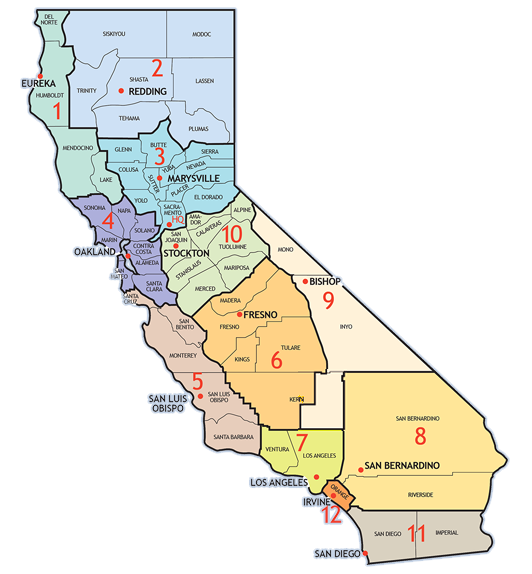
\includegraphics[scale=0.5]{images/caltrans-district-map.png}
	\caption{Caltrans District Map\protect\footnotemark}
	\label{fig:caltrans-map}
\end{figure}

\footnotetext{\url{https://dot.ca.gov/caltrans-near-me}}

\subsubsection{COVID-19}

The COVID-19 data is hosted on GitHub. Collecting the data is as simple as executing a \mintinline{bash}{git clone} command and refreshing the data is achieved with the \mintinline{bash}{git pull} command.

\subsection{Data Environment}
\label{sec:data-env}

The data environment employs the Amazon Web Services (AWS)\footnote{\url{https://aws.amazon.com/}} ecosystem for storing raw and processed data. The raw data from the sources discussed in Section \ref{sec:data-sources} are organized in an Amazon Simple Storage Service (S3)\footnote{\url{https://aws.amazon.com/s3/}} bucket to ensure the processed data can be recreated on demand without the need to download the raw data. Once the S3 bucket is initially populated, the intended goal of the PeMS scraper described in Section \ref{sec:data-collect-traffic} is that it is only used to download new data as it becomes available. The raw data consists of daily PeMS traffic files from each Caltrans district and the COVID-19 CSV files.

The daily raw traffic files are then processed (see Section \ref{sec:data-prep}) and stored in a PostgreSQL database hosted on Amazon Relational Database Service (RDS)\footnote{\url{https://aws.amazon.com/rds/}} to permit easy access for all team members and enable online processing for deployed models. This interface allows the team to set up and run workflows either locally or on a cloud compute infrastructure. The team connects to and interacts with the database using either Python libraries (e.g. SQLAlchemy or psycopg2) or Jupyter SQL magic functions inside a Jupyter notebook. This enables easy execution of SQL commands to add processed data to the database (\mintinline{text}{INSERT}), modify existing records (\mintinline{text}{UPDATE}), or to query desired data for analysis (\mintinline{text}{SELECT}).

The traffic tables in the RDS database contain station measurements (speed, number of vehicles, etc.) at five-minute intervals, as well as and station metadata (coordinates, freeway number/direction, etc.). Even though the COVID-19 data simply consists of two small CSV files, it was also added to the database in order to have all data in a unified location. Since both the Caltrans and COVID-19 data sources are updated daily, a cron job can be utilized to fetch the latest data, perform required processing, and store it in the database.

\subsection{Data Pipeline}
\label{sec:data-pipeline}

The data pipeline is illustrated in Figure \ref{fig:data-pipeline} below. It shows the traffic and COVID-19 data being fetched as described in Section \ref{sec:data-collect} and stored in S3 buckets. Once the data resides on S3, it is processed and inserted to the appropriate tables in the RDS database. Finally, the processed data is pulled from the database for analysis, including EDA and machine learning.

\begin{figure}[hbt!]
	\centering
	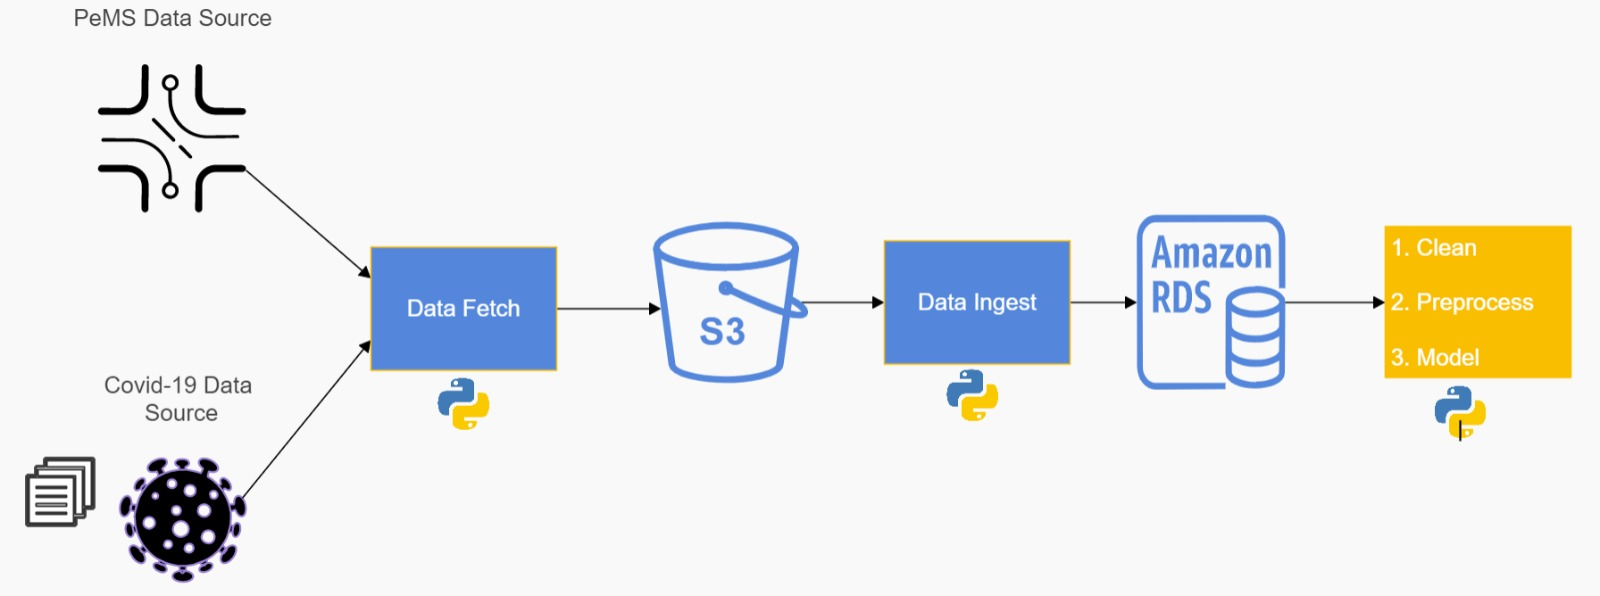
\includegraphics[width=\textwidth]{images/data-pipeline-new.jpeg}
	\caption{Data Pipeline}
	\label{fig:data-pipeline}
\end{figure}

\section{Data Preparation}
\label{sec:data-prep}

Data preparation is performed during both the data ingest and final steps in the data pipeline presented above in Section \ref{sec:data-pipeline}. During data ingestion, each daily traffic file is processed prior to being stored in the database. The data is very clean overall as it is organized by Caltrans and Johns Hopkins University and fortunately requires little preprocessing. Even though Caltrans provides traffic data in daily files, there are occasional instances where a given file contains additional data from the previous day. To account for this, the data is filtered on the timestamp column to only contain data from the appropriate day before entry to the database.

Additional preprocessing steps required for making traffic forecasts are to handle missing values and arrange the data in the form expected by the given model, such as with a sliding window, rolling average, etc. However, since this process varies by model, these data preparation steps are performed once the desired traffic data (i.e. region, time frame, etc.) is selected from the database, rather than selecting a fixed methodology and applying it to the processed data stored on RDS. While the PeMS data is clean, there are intermittent missing rows. Missing timestamps are populated with nearby values since the data does not typically change drastically between timestamps. Since the database stores traffic measurements from all stations in the same column (e.g. all speeds are in the same column), one must use care to ensure measurements from stations are not mixed during analysis. Once the desired data is read from the database into a pandas \mintinline{python}{DataFrame}, stations can be separated with the \mintinline{python}{pivot} method.

\begin{minted}{python}
traffic.pivot(index="timestamp", columns="station", values="avg_speed")
\end{minted}

This creates a matrix of average speed values organized by time along rows and traffic stations across columns. From there the data can be structured for each model, such as creating rolling windows for each station to predict speed at a given time based on previous measurements.

\section{Analysis Methodology}

The analysis methodology consists of initial data analysis to understand the data and model development for time series forecasting. In addition to traffic forecasting, we performed some COVID-19 forecasting to help support library development.

\subsection{Exploratory Data Analysis (EDA)}

Once we had robust data pipeline developed, we explored the data we had at our disposal to analyze the structure of the data and discover underlying trends.

\subsubsection{Traffic}

The Caltrans PeMS standard rollup provides a variety of measurements (number of vehicles, average speed, etc.) for both individual lanes and across all lanes in five-minute intervals aggregated from the raw 30-second intervals. Regular periods of high traffic (i.e. rush hour) are the timeframes most greatly impacted by fewer vehicles on the road. Figure \ref{fig:traffic-eda-day} below displays average vehicle speed between 4-7 PM across all stations in Caltrans District 4, which encompasses the San Francisco Bay Area. There is a noticeable increase in average speed beginning mid-March when COVID-19 began to greatly impact the United States and the fluctuations between weekday and weekend speeds are much smaller compared to pre-COVID traffic.

\begin{figure}[hbt!]
	\centering
	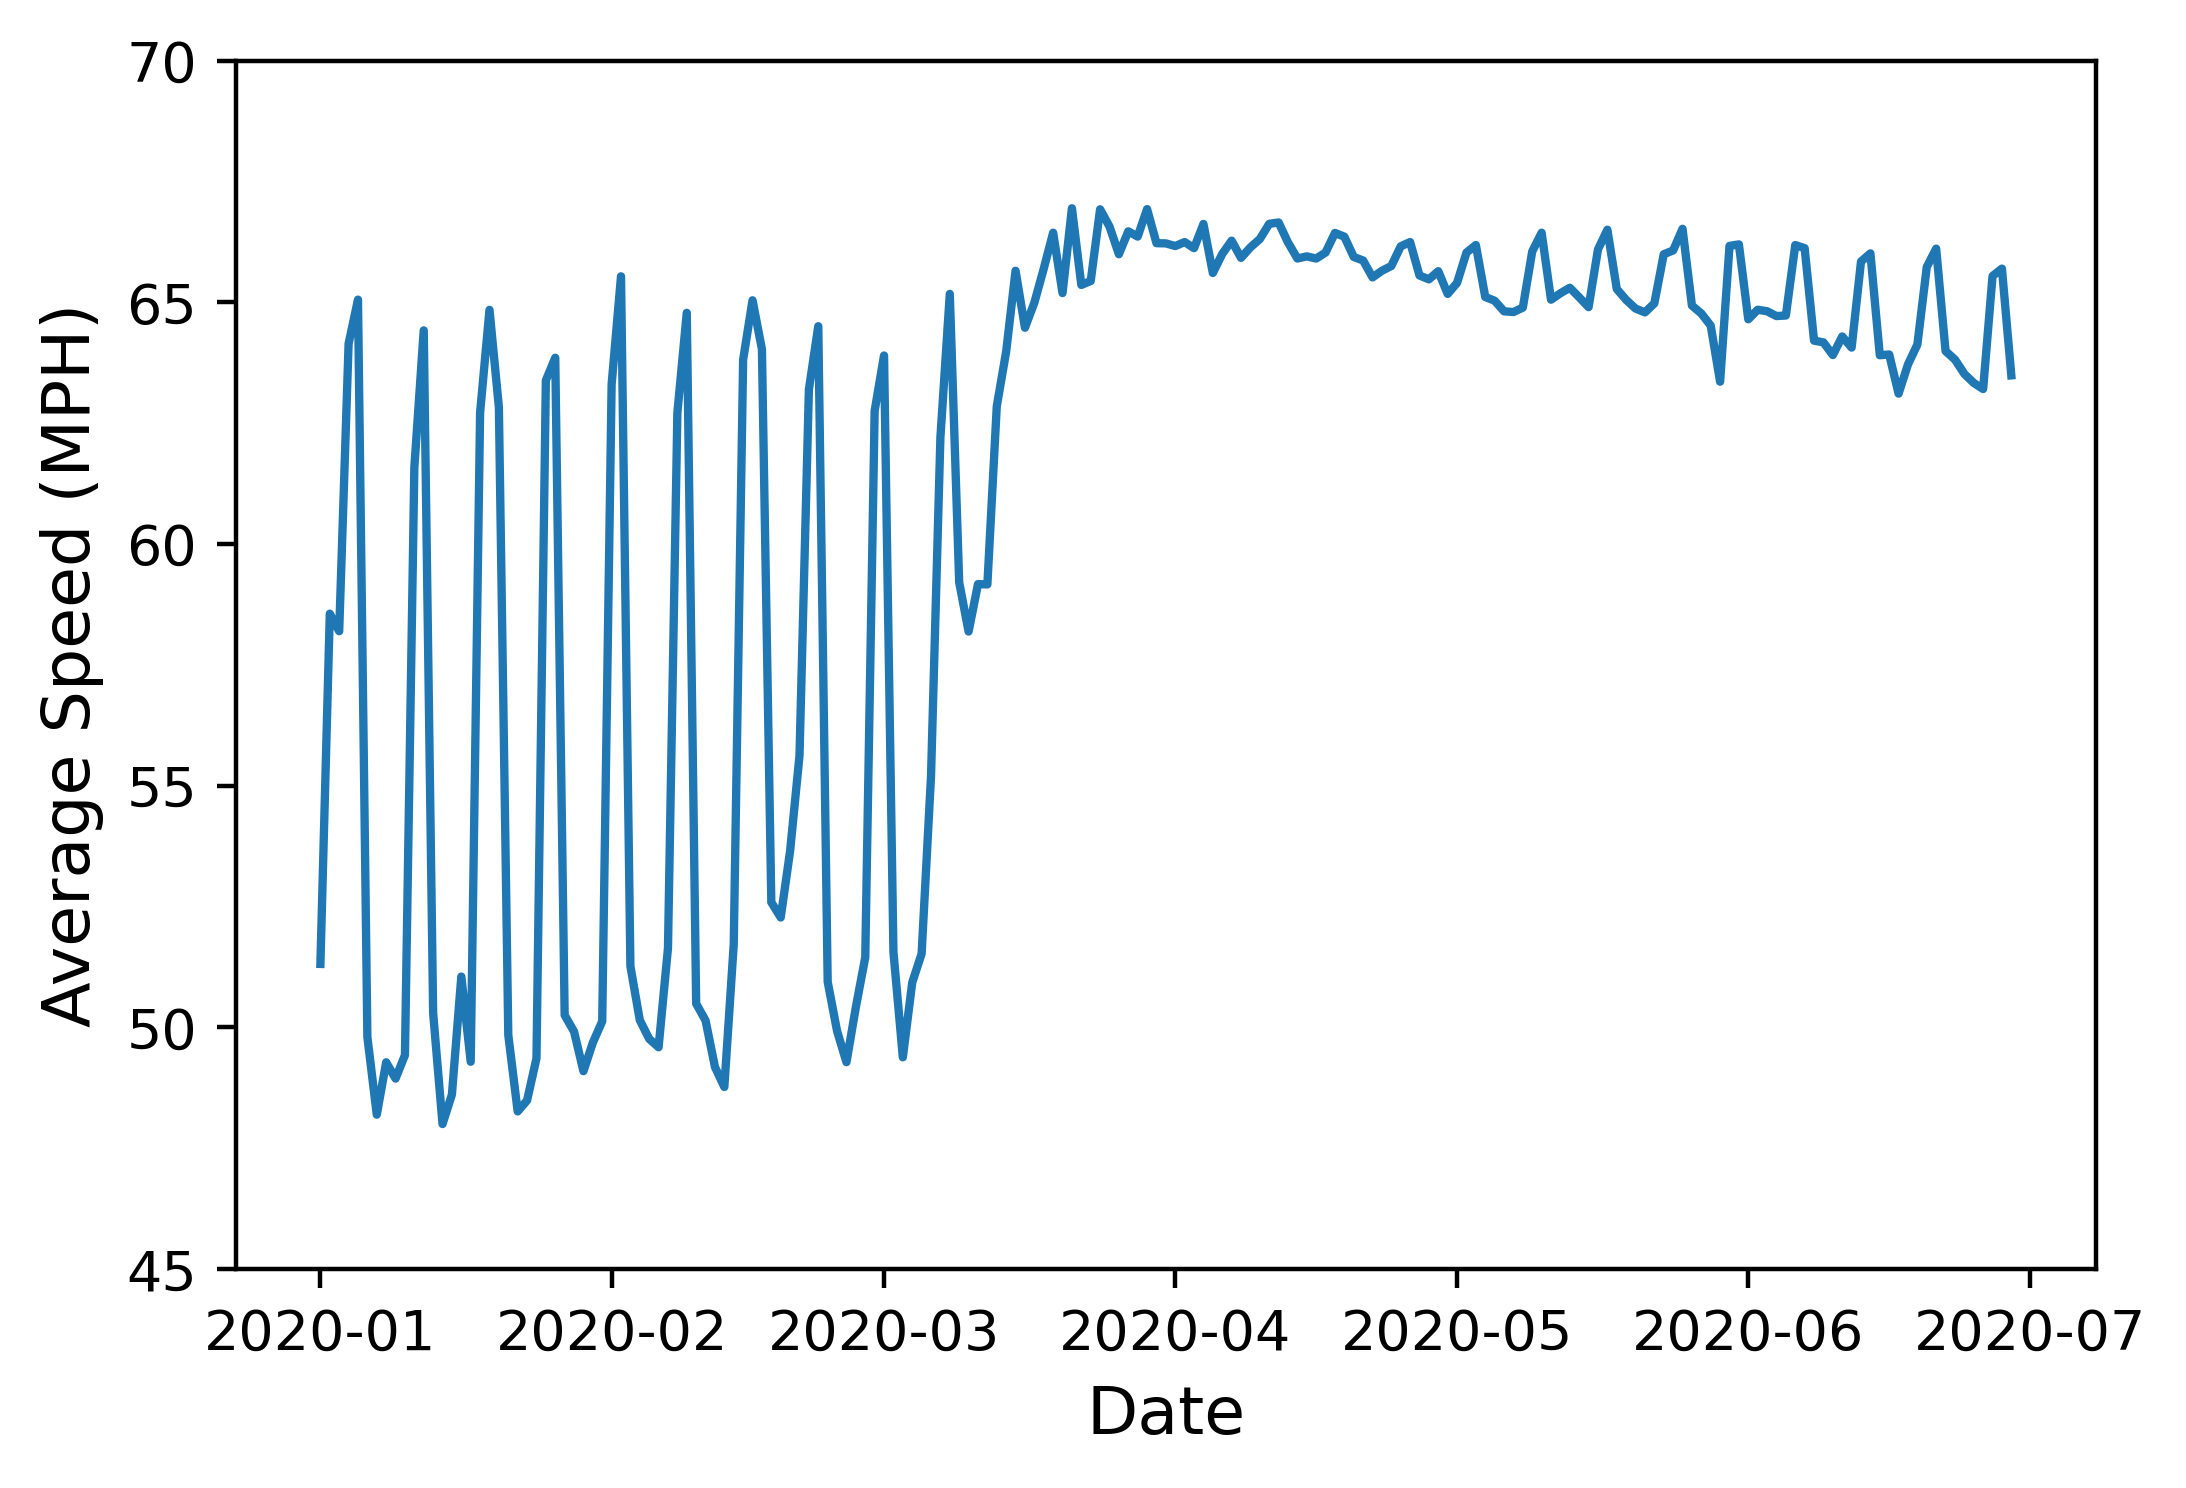
\includegraphics[width=0.6\textwidth]{images/traffic_speed_day.png}
	\caption{Average vehicle speed during evening rush hour (4-7 PM) in PeMS district 4.}
	\label{fig:traffic-eda-day}
\end{figure}

Figure \ref{fig:traffic-eda-month} below presents an average day of traffic during January and April 2020 in Caltrans District 4 with average vehicle speed on the left in Figure \ref{fig:traffic-eda-month-speed} and ``total flow'' (vehicles/5 min) on the right in Figure \ref{fig:traffic-eda-month-flow}. It illustrates that traffic was much lighter throughout the day in April with the largest differences occurring during the morning and evening rush hours, which are essentially nonexistent in April. Average speed during the early morning and late evening hours are nearly identical between the two months since few vehicles are typically on the road at this time, pandemic or not. There is a large decrease in the number of vehicles on the road, particularly after roughly 5:00 AM.

\begin{figure}[hbt!]
    \centering
    \begin{subfigure}[b]{0.48\textwidth}
        \centering
        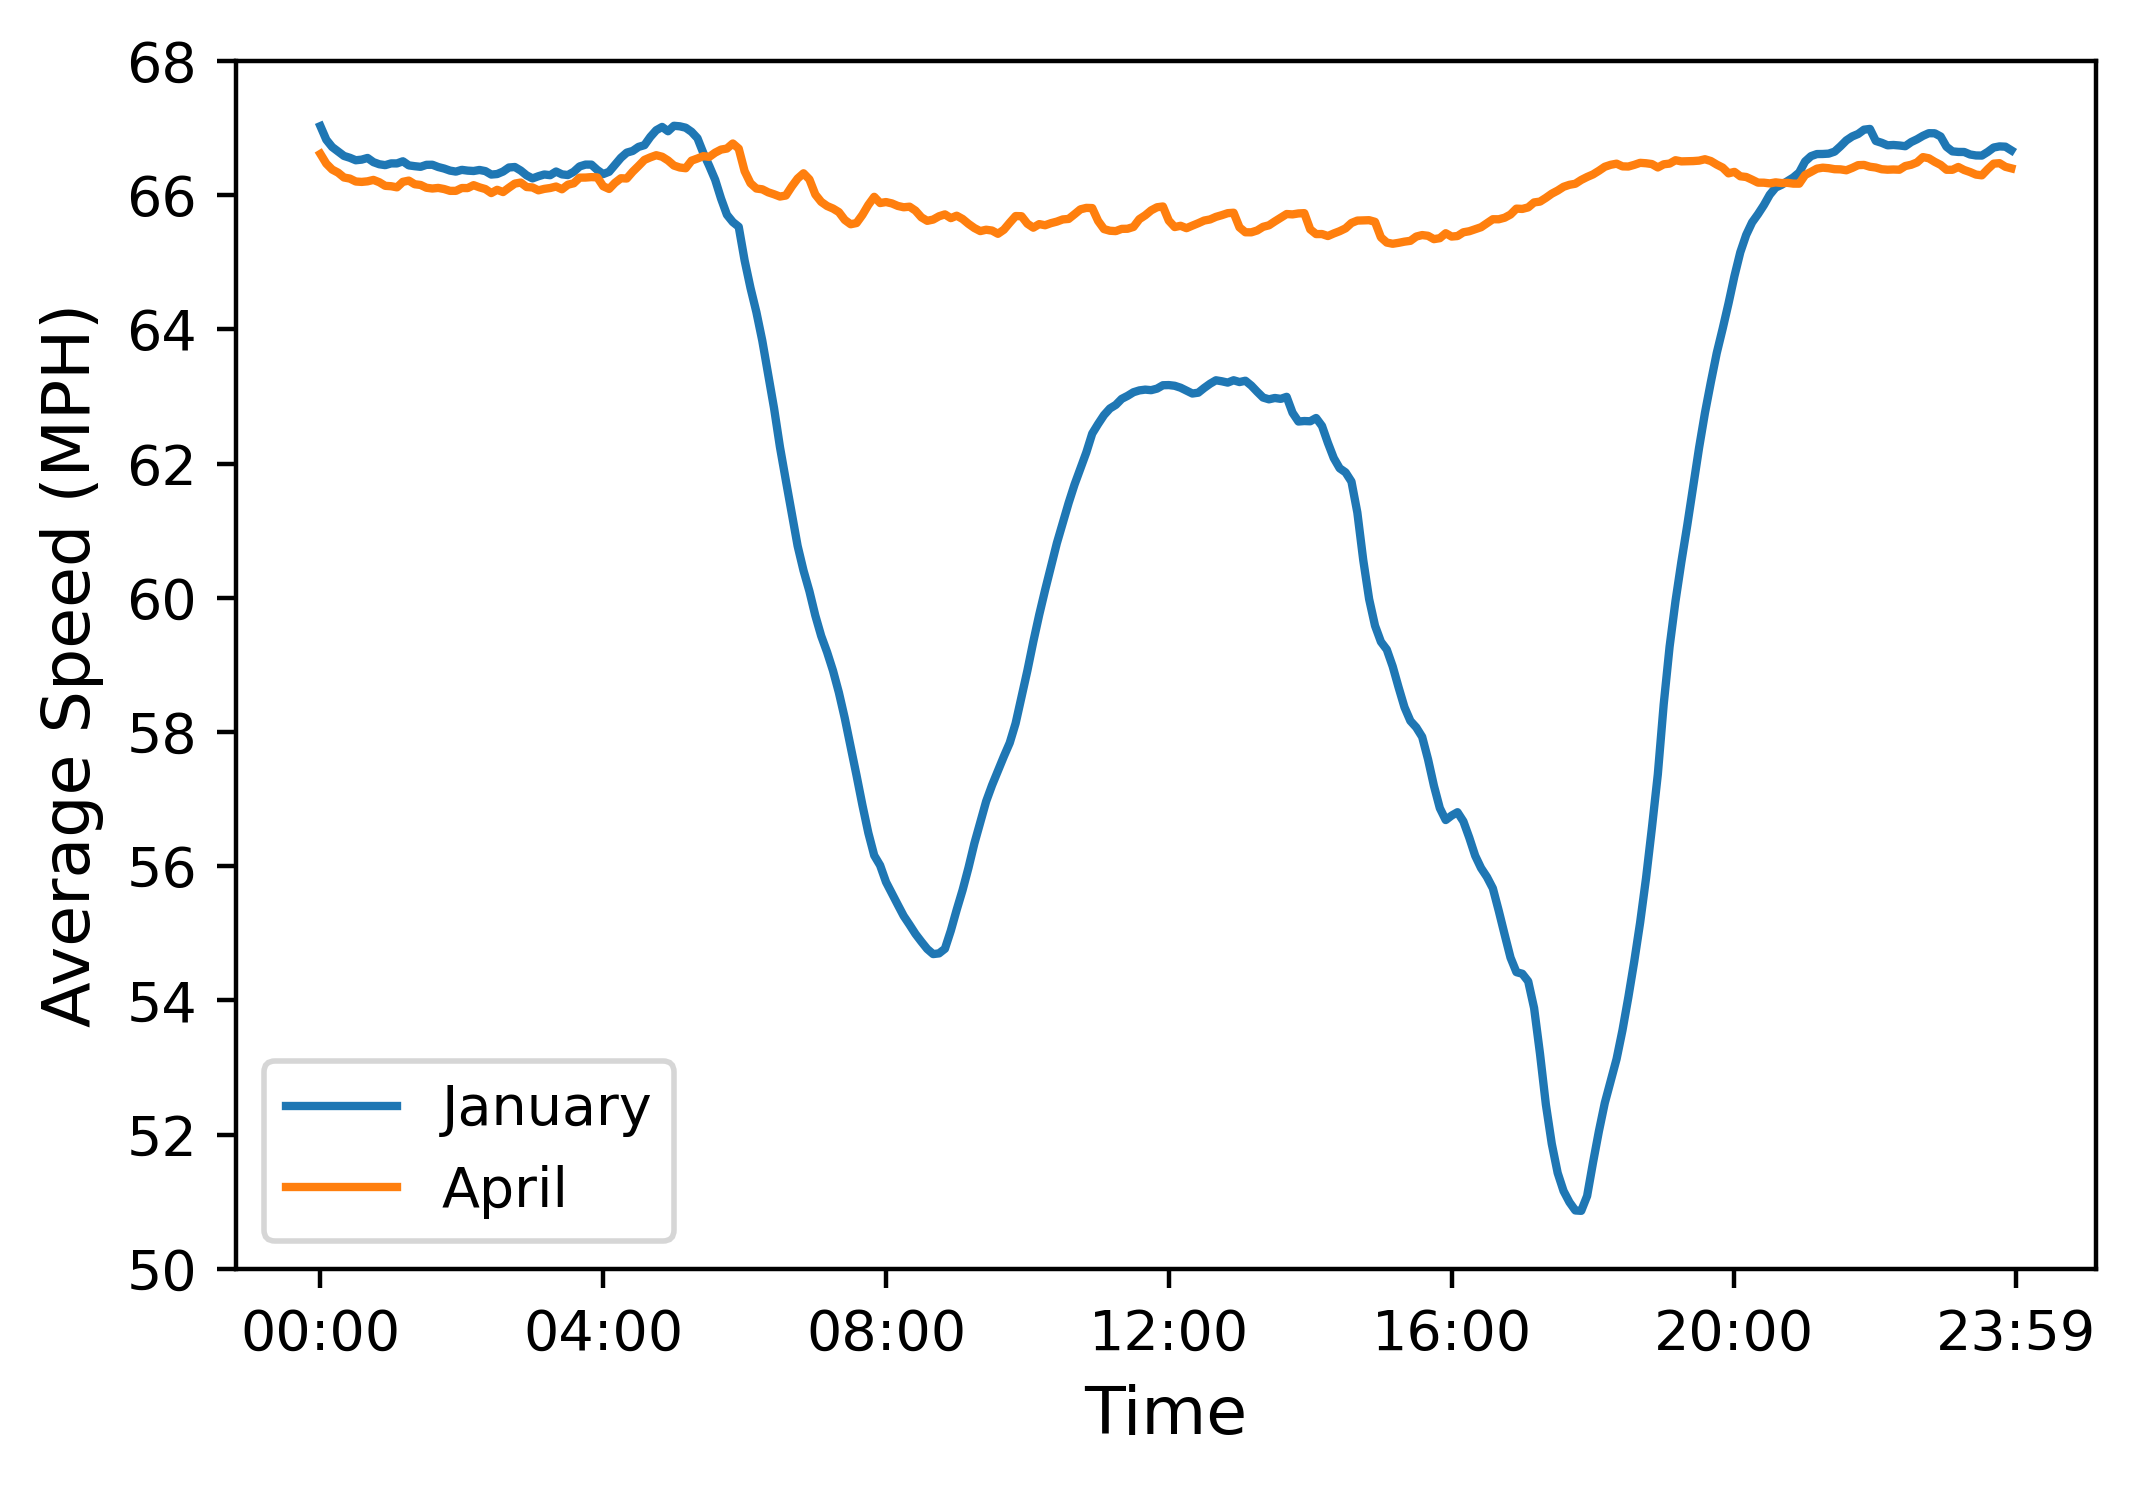
\includegraphics[width=\textwidth]{images/traffic_speed.png}
        \caption{Average vehicle speed}
        \label{fig:traffic-eda-month-speed}
    \end{subfigure}
    \hfill
    \begin{subfigure}[b]{0.48\textwidth}
        \centering
        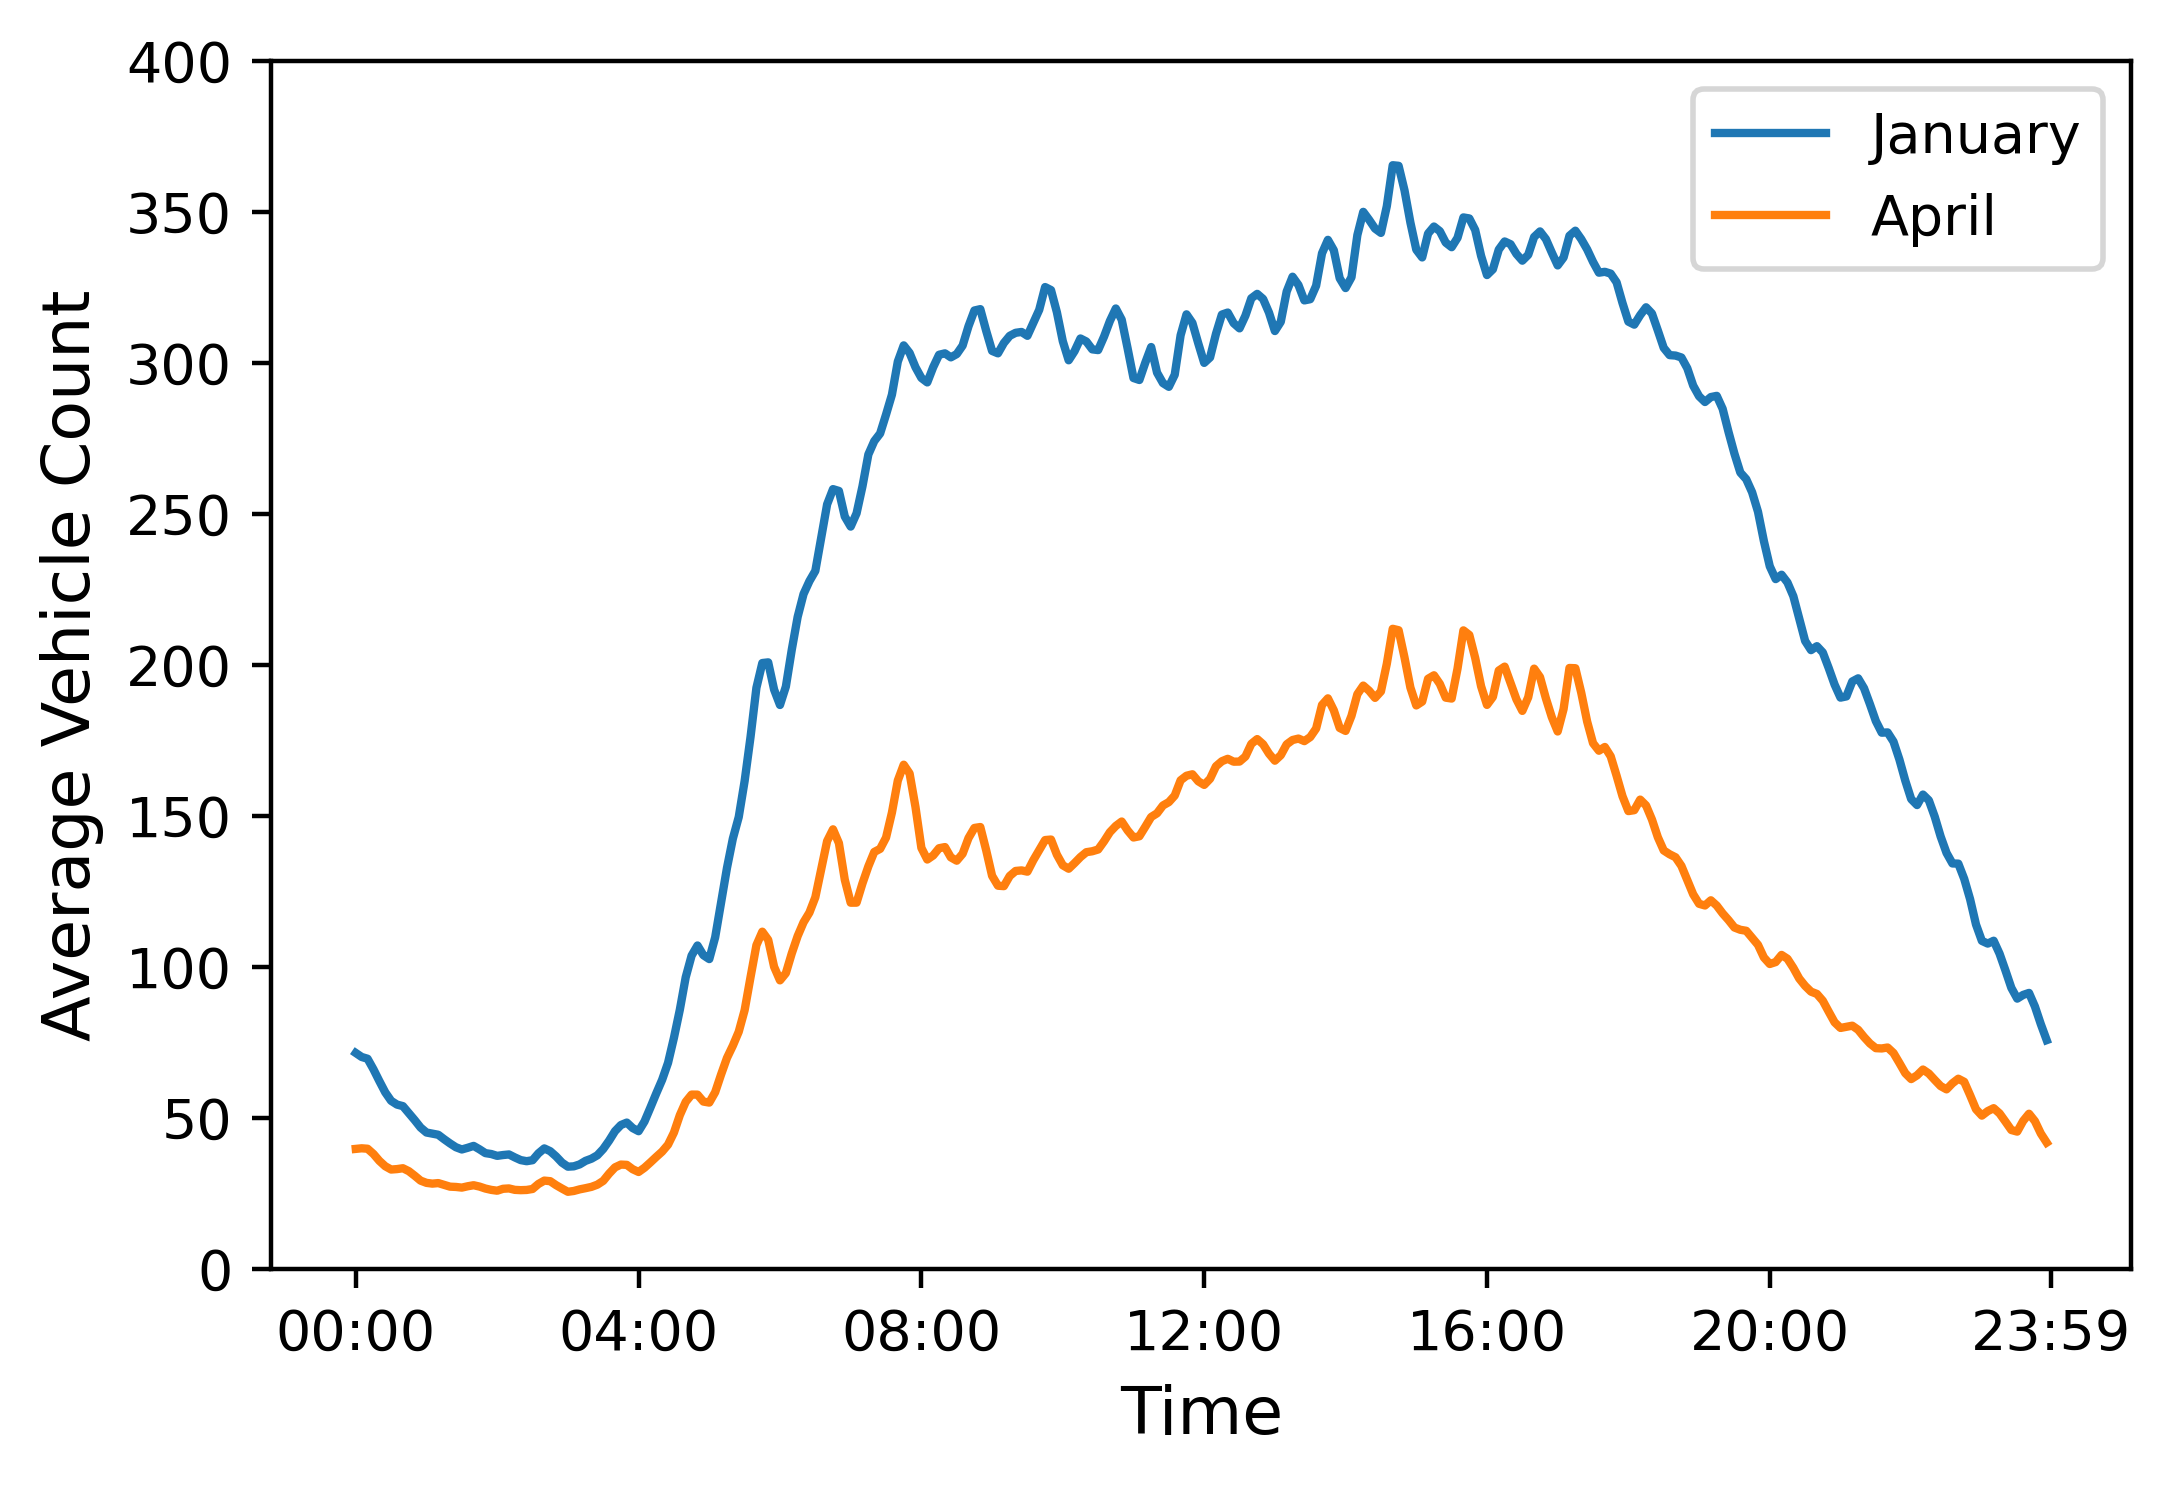
\includegraphics[width=\textwidth]{images/traffic_flow.png}
        \caption{Average number of vehicles}
        \label{fig:traffic-eda-month-flow}
    \end{subfigure}
    \caption{Comparison of traffic patterns between Jan and April 2020 in PeMS district 4.}
    \label{fig:traffic-eda-month}
\end{figure}

\subsubsection{COVID-19}

The COVID-19 dataset provides the cumulative total number of cases for a given day and county in the United States. The left graph in Figure \ref{fig:covid-eda} below displays the raw data for the top 6 counties in California, which illustrates that Los Angeles County dwarfs the other top counties in California with over 4 times as many cases. There is also a precipitous drop after counties 2-5 as Santa Clara County has fewer than half the number of cases as San Bernardino, Riverside, Orange, and San Diego counties. The right graph provides the number of new cases, which is simply the difference from the previous day in the cumulative distribution. These values are occasionally negative and are possibly caused by over-counting or false positives from a previous day. 

\begin{figure}[hbt!]
    \centering
    \begin{subfigure}[b]{0.48\textwidth}
        \centering
        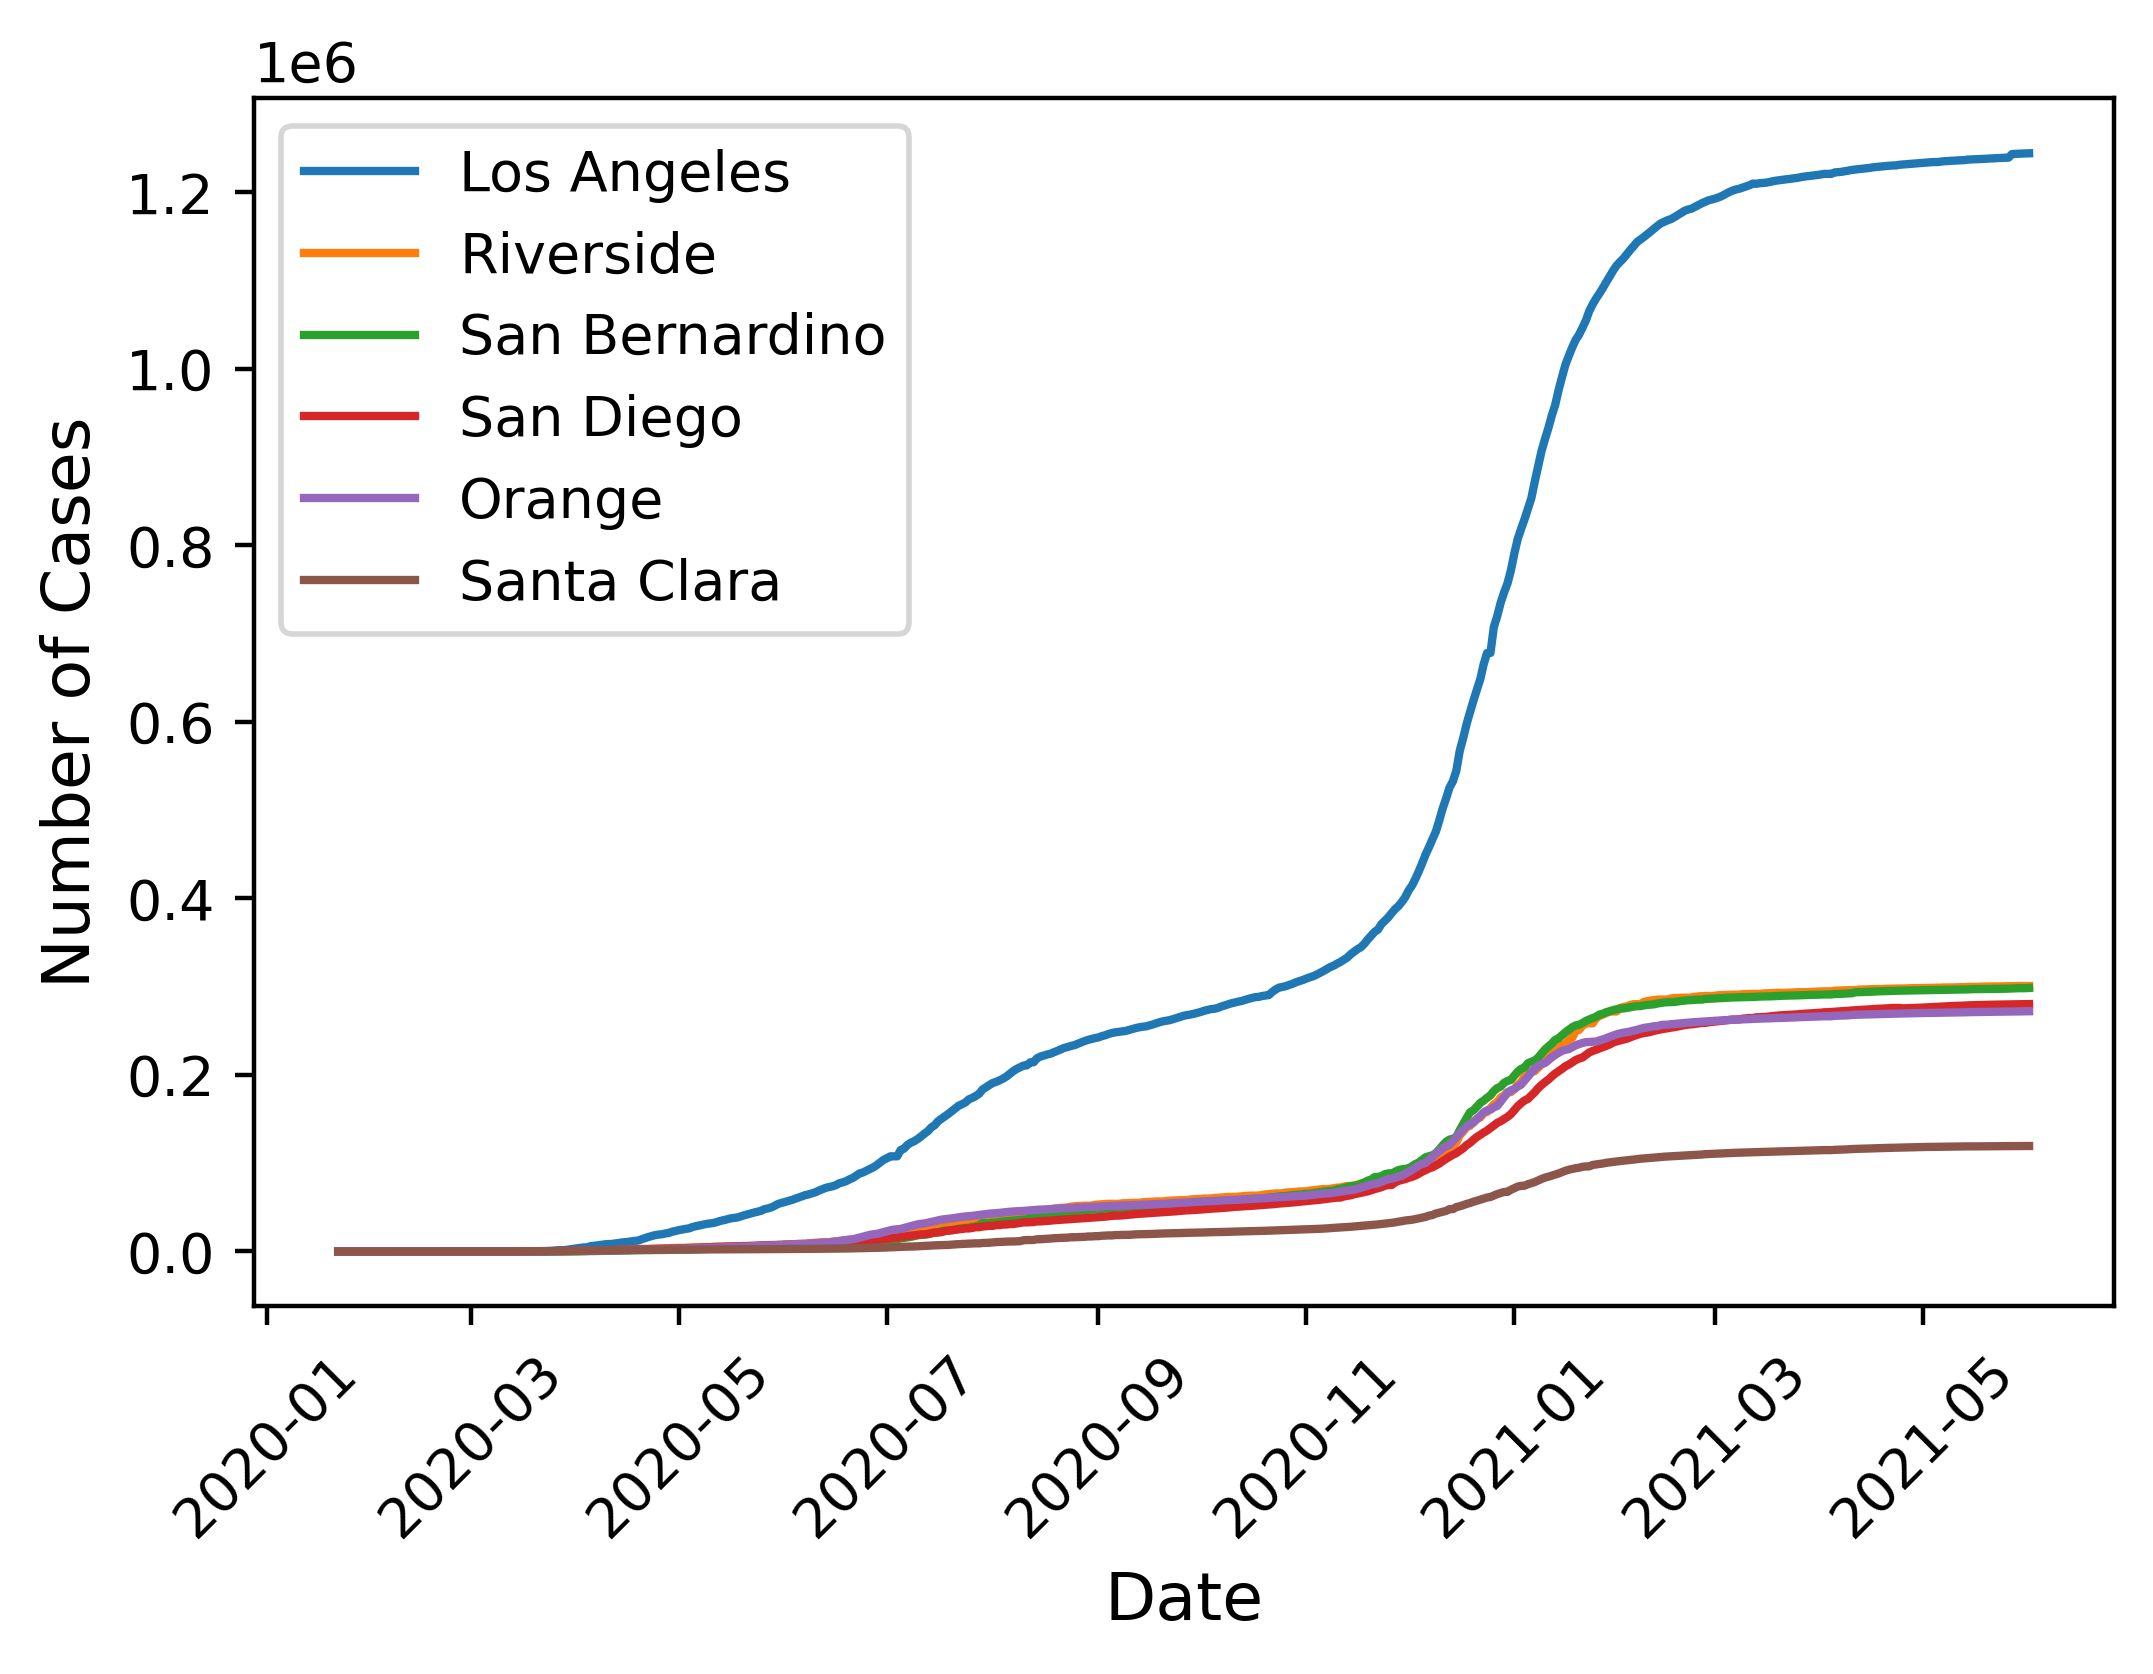
\includegraphics[width=\textwidth]{images/covid_cases_ca_county_cumulative.png}
        \caption{Cumulative}
        \label{fig:traffic-eda-cumulative}
    \end{subfigure}
    \hfill
    \begin{subfigure}[b]{0.48\textwidth}
        \centering
        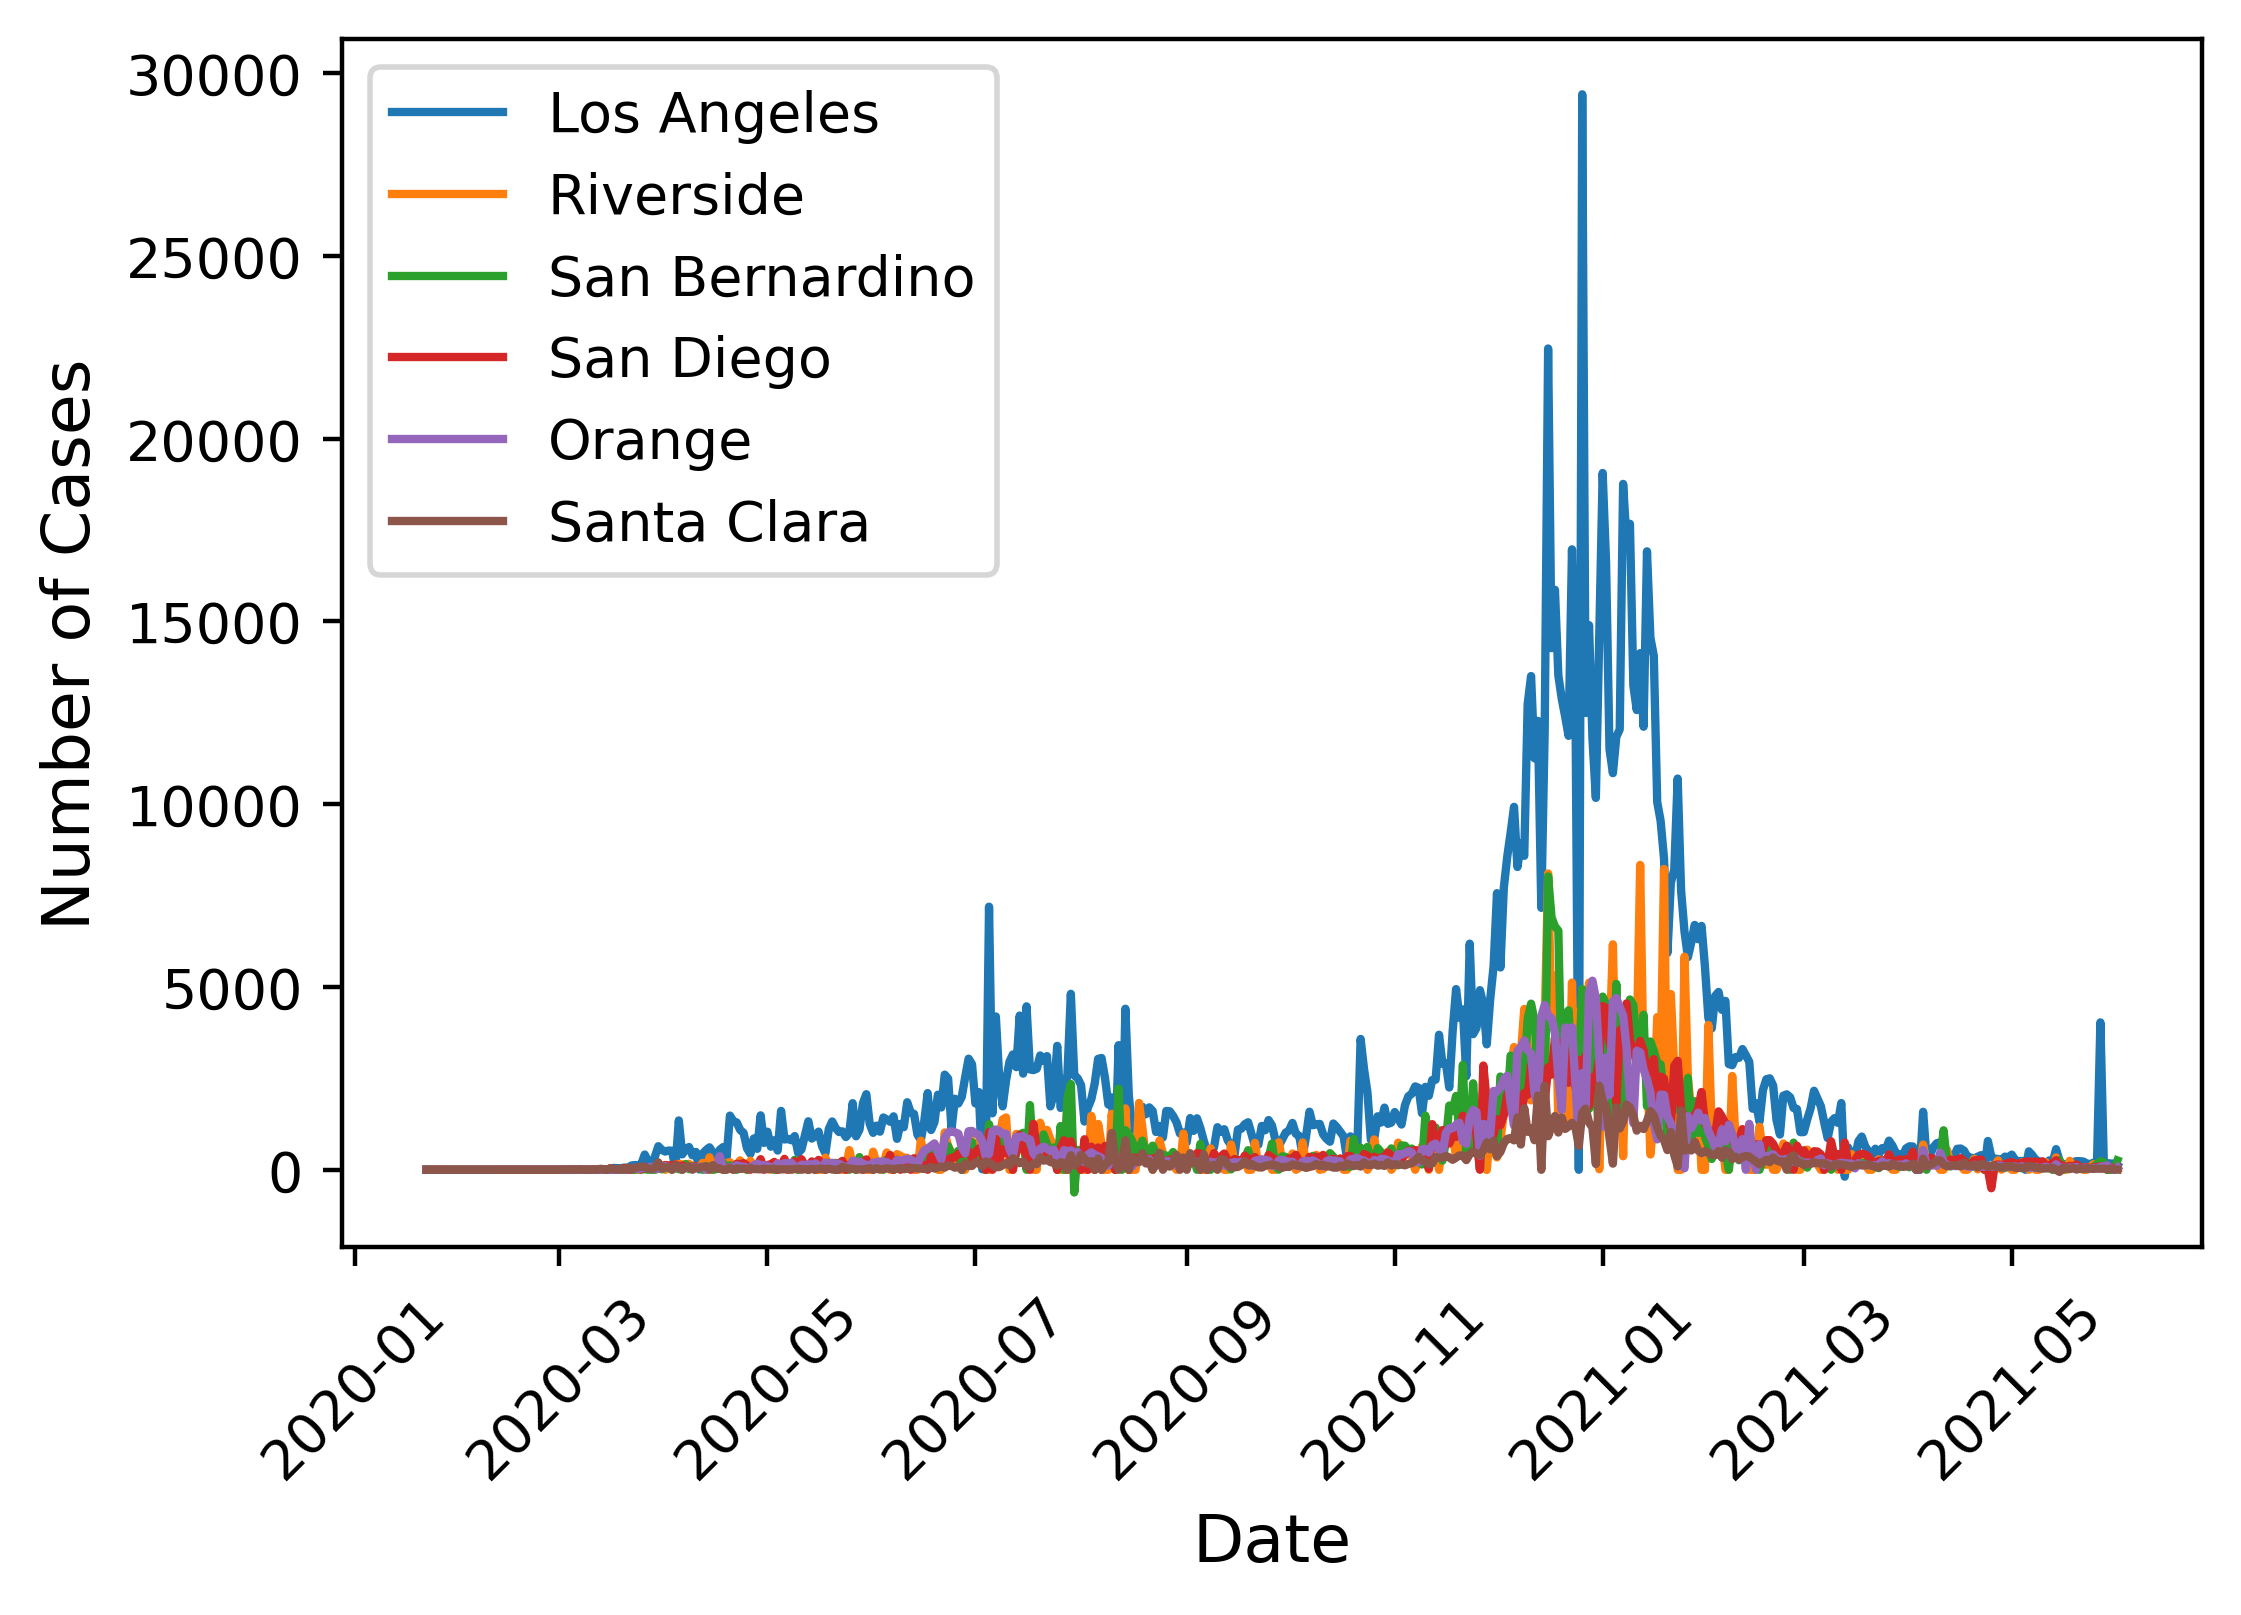
\includegraphics[width=\textwidth]{images/covid_cases_ca_county_daily.png}
        \caption{Daily}
        \label{fig:covid-eda-daily}
    \end{subfigure}
    \caption{COVID-19 Cases in California (Top 6 Counties by Total Cases)}
    \label{fig:covid-eda}
\end{figure}

% \begin{figure}[hbt!]
% 	\centering
% 	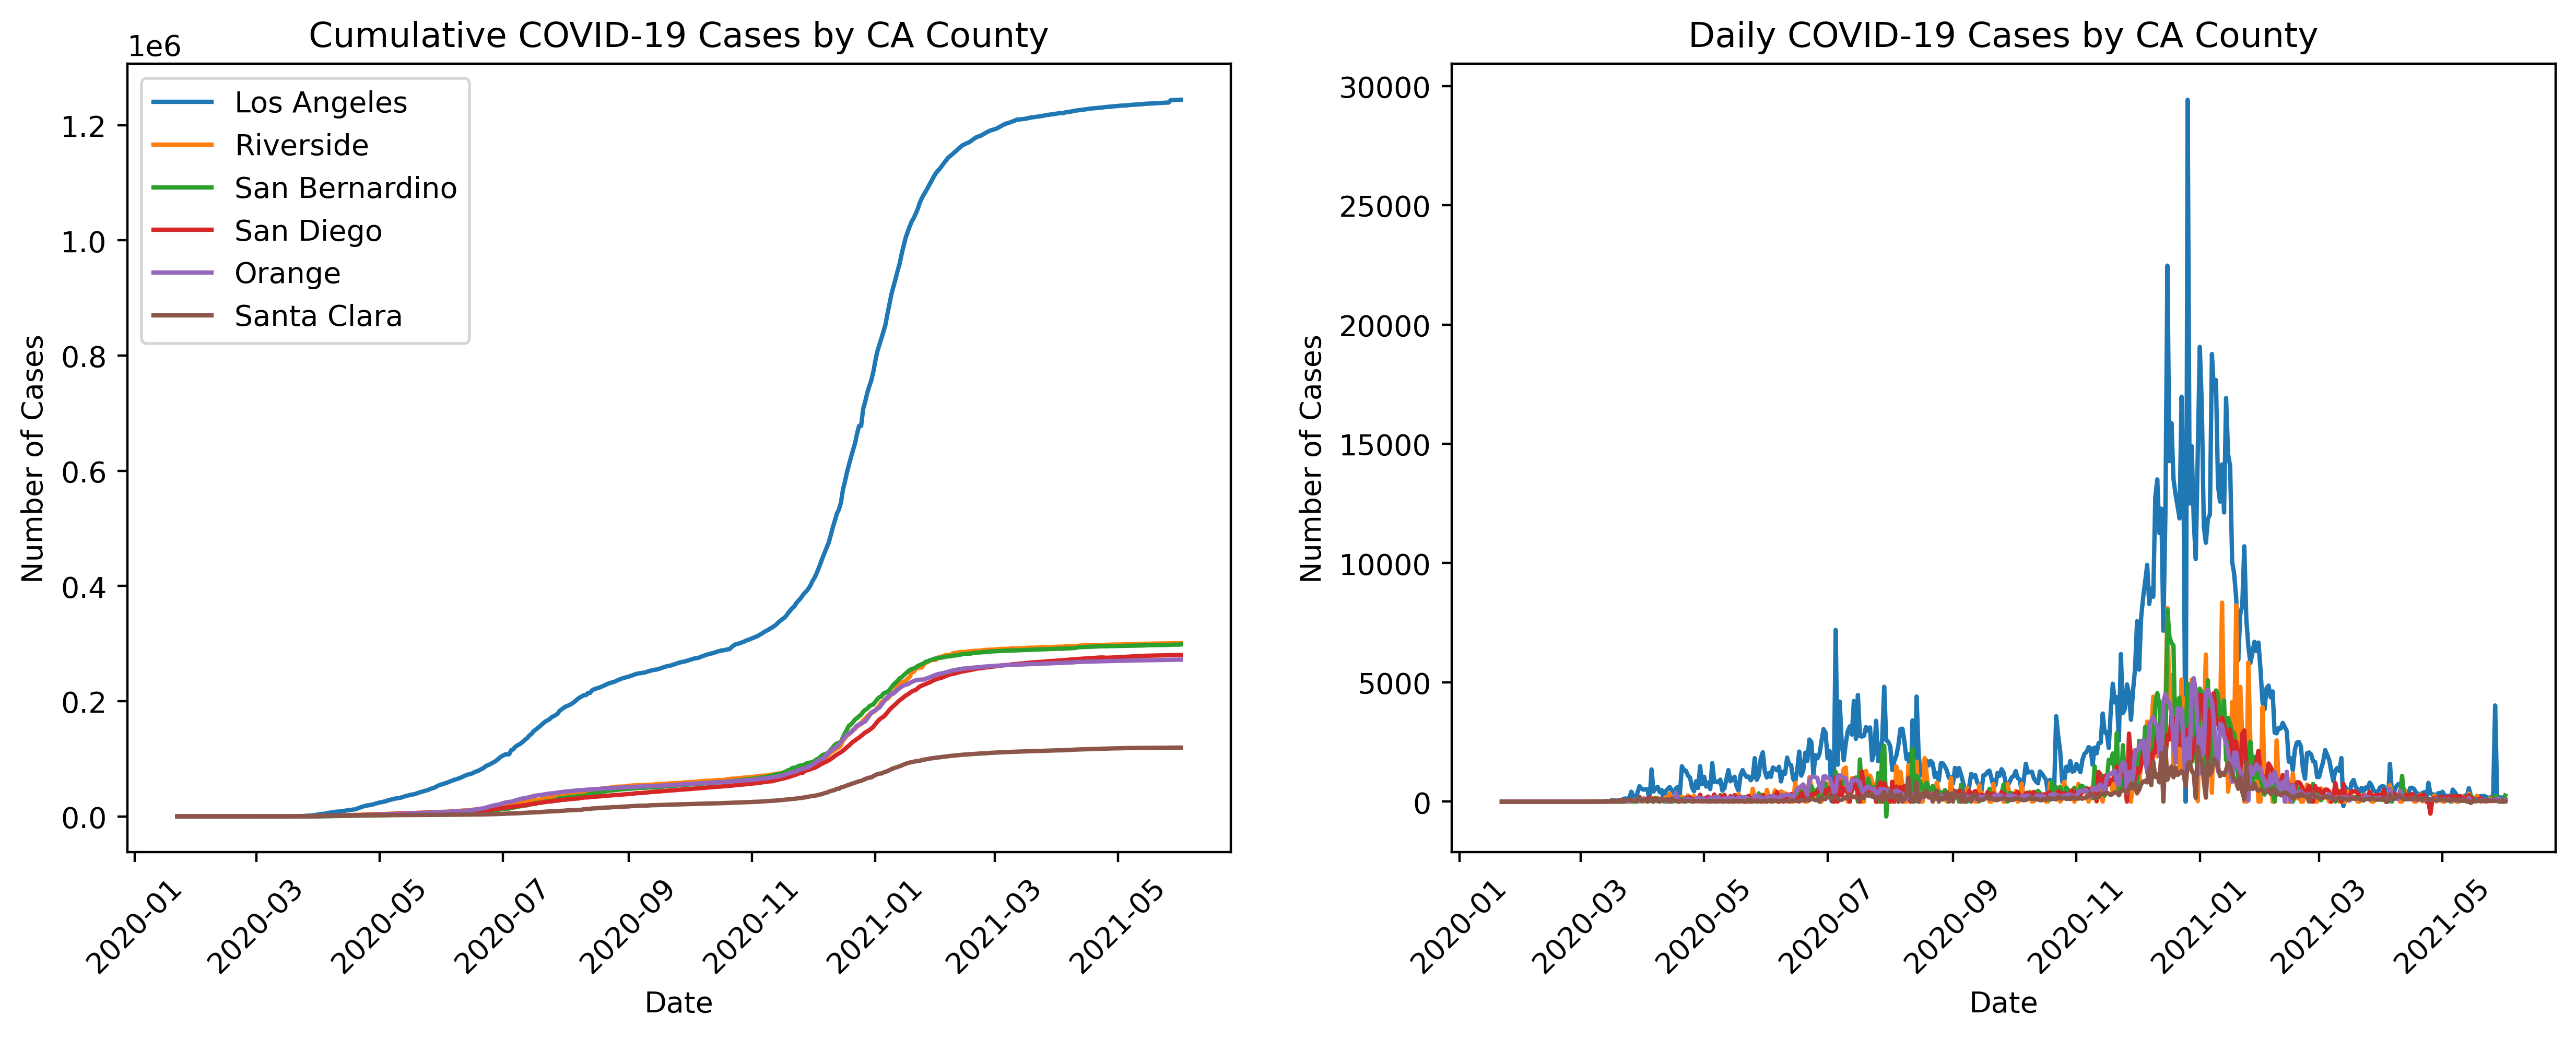
\includegraphics[width=\textwidth]{images/covid_cases_ca_county.png}
% 	\caption{COVID-19 Cases in California (Top 6 Counties by Total Cases)}
% 	\label{fig:covid-eda}
% \end{figure}

However, the figure above can be misleading given that Los Angeles County has more than 3 times as many residents as any other county in California.\footnote{\url{https://en.wikipedia.org/wiki/List_of_counties_in_California}} Figure \ref{fig:covid-eda-per-capita} below displays the same data after normalizing the case numbers by population. It shows that San Bernardino County has the highest case rate per capita, but with a population of roughly 2.2 million compared to LA’s over 10 million, San Bernardino compares favorably in absolute terms.

\begin{figure}[hbt!]
    \centering
    \begin{subfigure}[b]{0.48\textwidth}
        \centering
        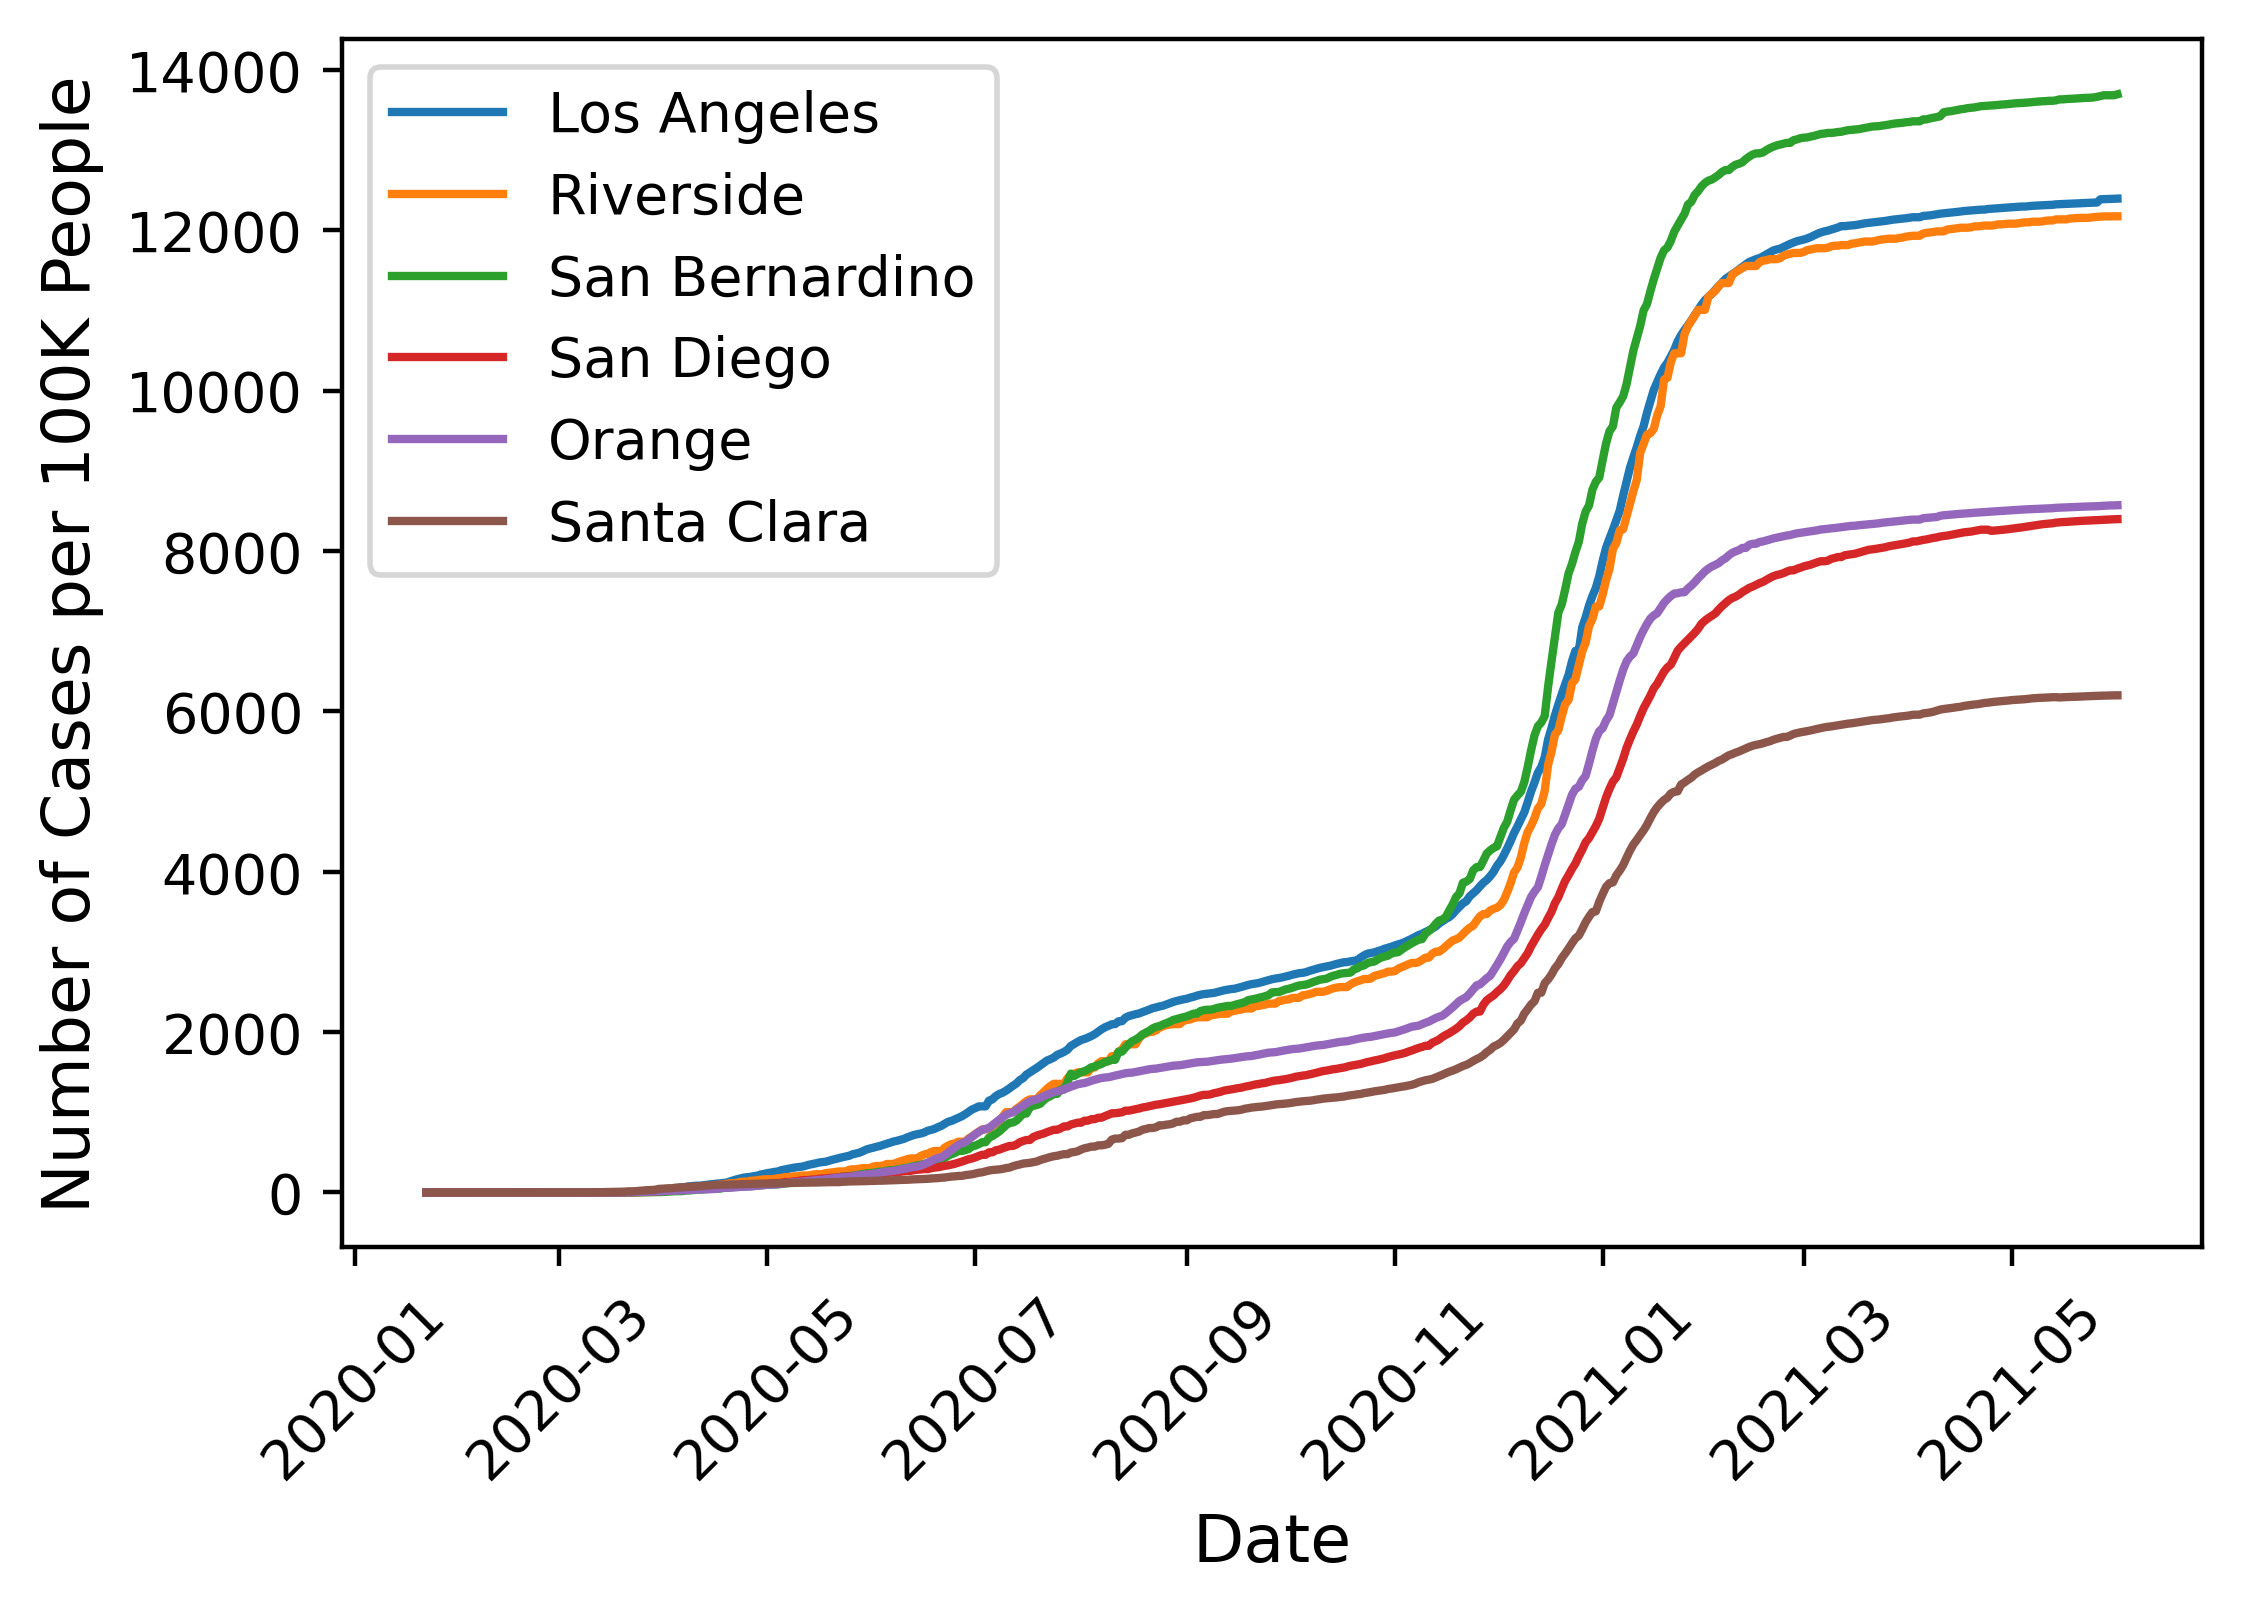
\includegraphics[width=\textwidth]{images/covid_cases_ca_county_cumulative_per_capita.png}
        \caption{Cumulative}
        \label{fig:traffic-eda-cumulative-per-capita}
    \end{subfigure}
    \hfill
    \begin{subfigure}[b]{0.48\textwidth}
        \centering
        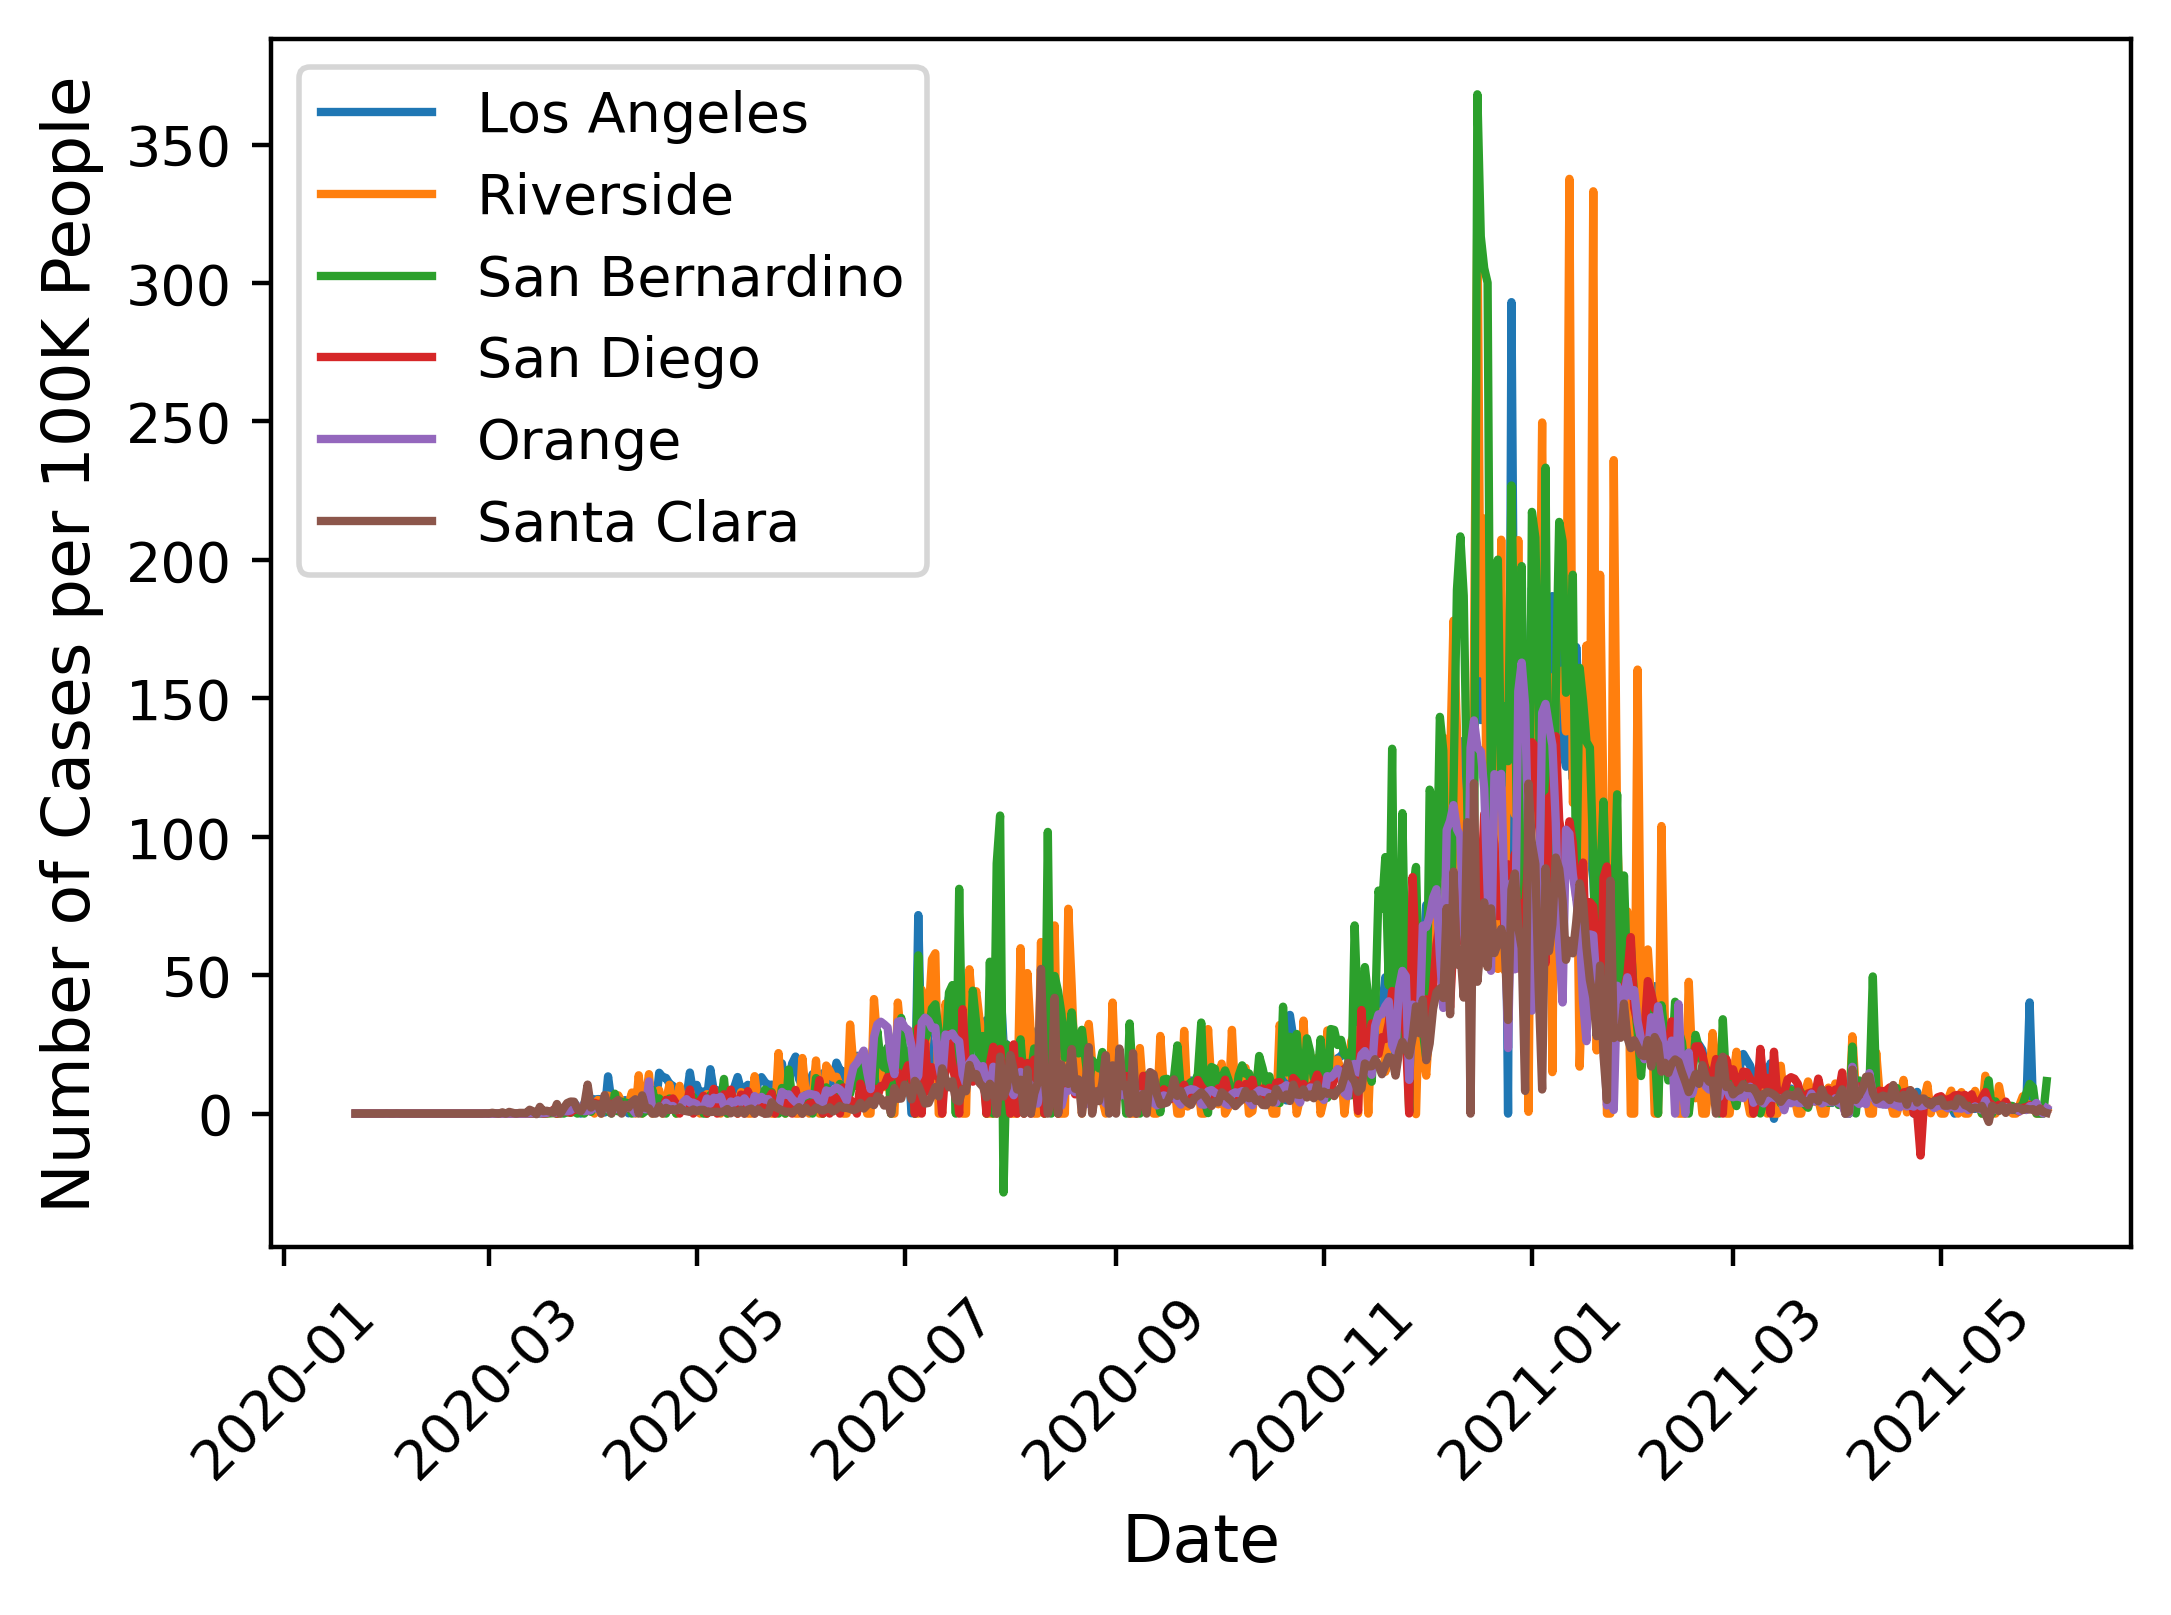
\includegraphics[width=\textwidth]{images/covid_cases_ca_county_daily_per_capita.png}
        \caption{Daily}
        \label{fig:covid-eda-daily-per-capita}
    \end{subfigure}
    \caption{COVID-19 Cases in California per 100K People (Top 6 Counties by Total Cases)}
	\label{fig:covid-eda-per-capita}
\end{figure}

% \begin{figure}[hbt!]
% 	\centering
% 	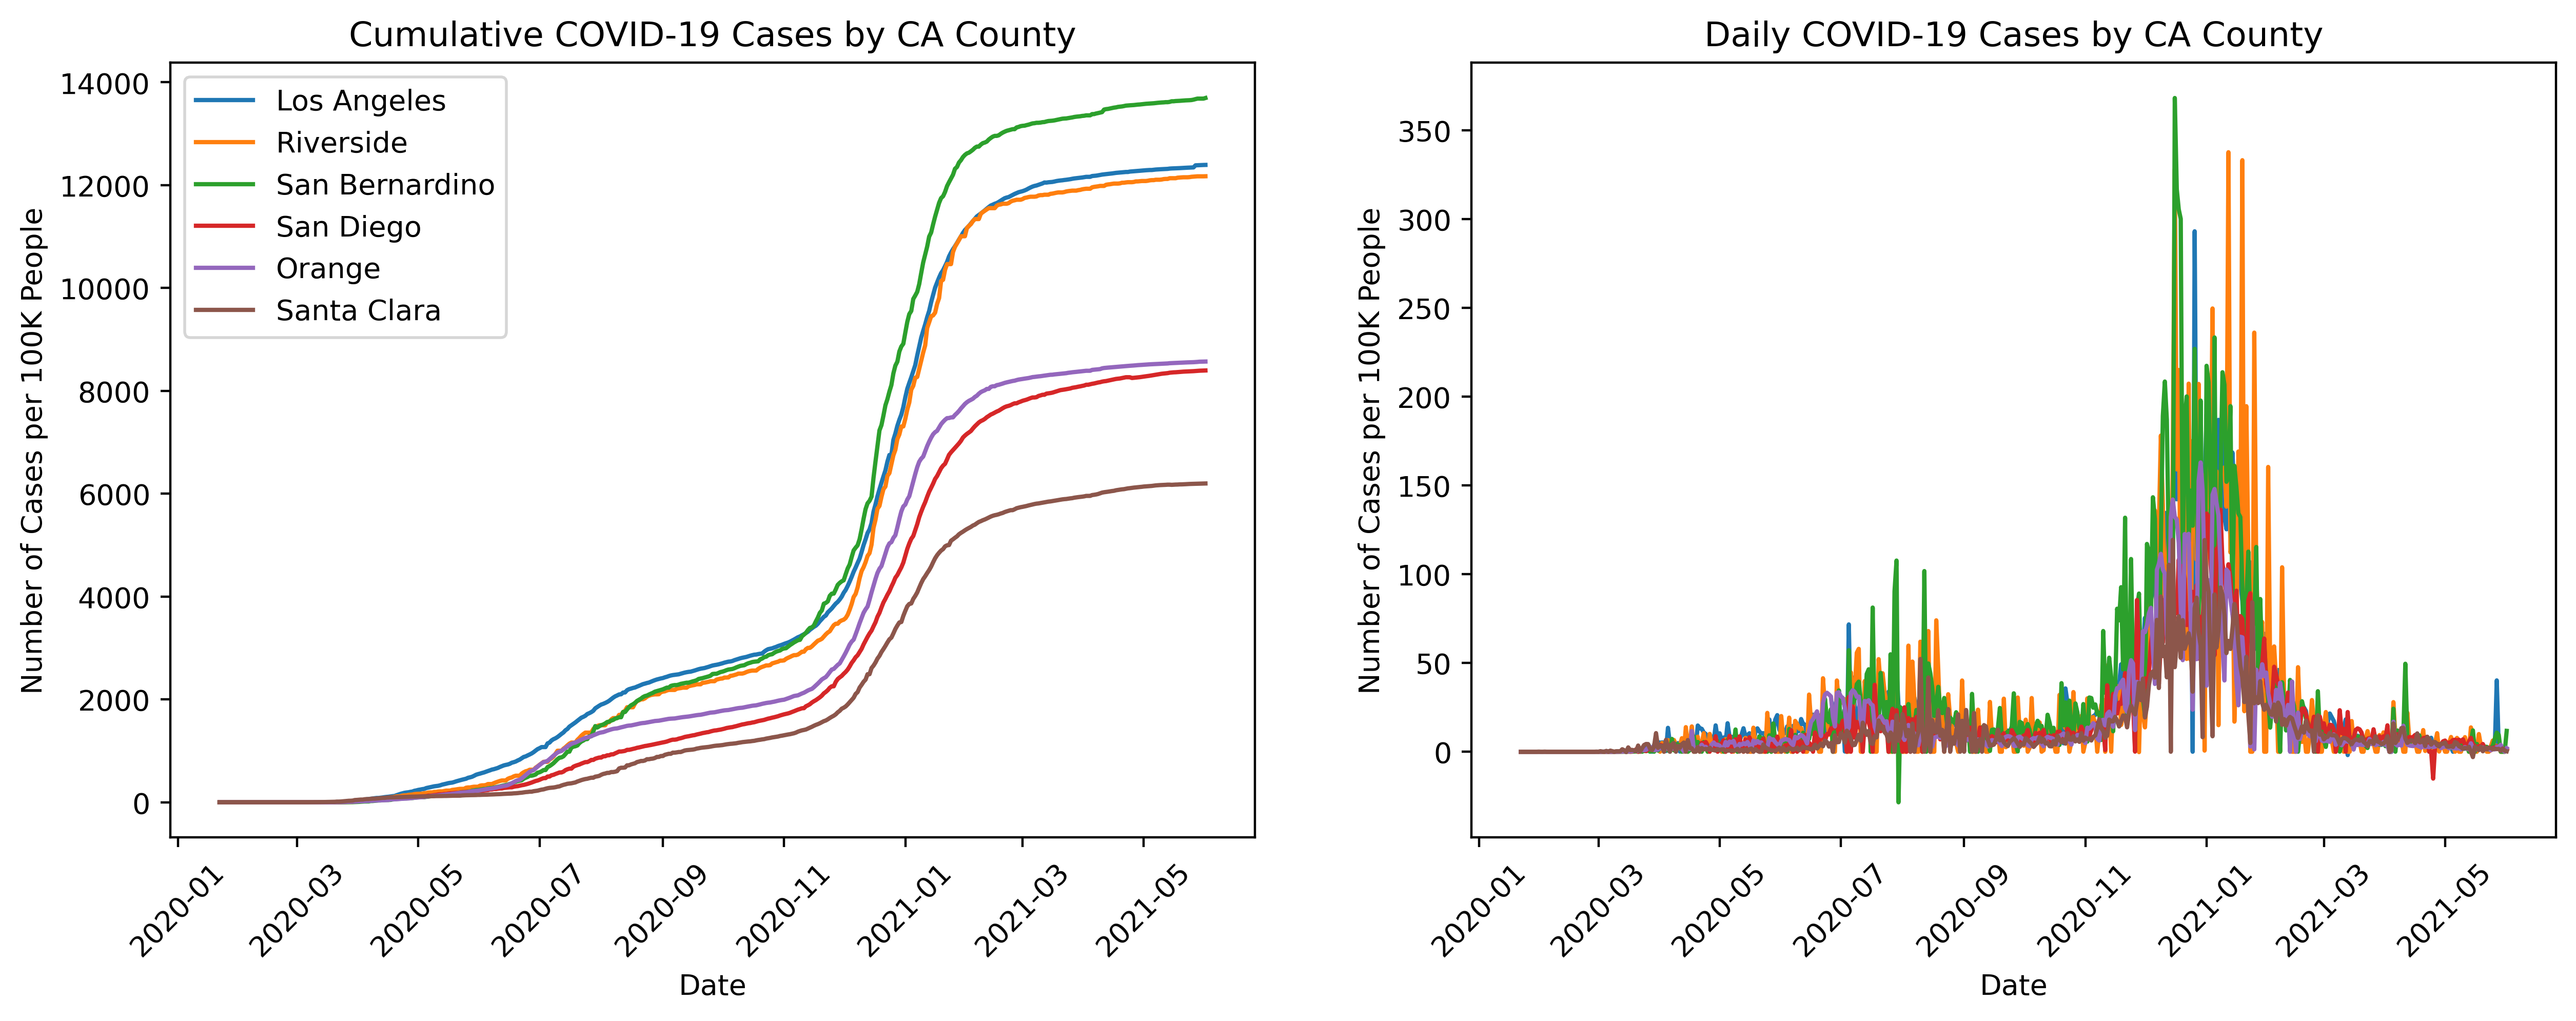
\includegraphics[width=\textwidth]{images/covid_cases_ca_county_per_capita.png}
% 	\caption{COVID-19 Cases in California per 100K People (Top 6 Counties by Total Cases)}
% 	\label{fig:covid-eda-per-capita}
% \end{figure}

\subsection{Models}
\label{sec:models}

There are four types of models developed for the deep learning time series library and applied to the problem of traffic forecasting. These are a classical time series model, spatiotemporal model, deep seq2seq, and a physics-informed neural network. The classical time series model is an autoregressive (AR) model implemented as a linear neural network with one hidden layer to better scale to large data compared to a traditional AR model. The spatiotemporal model is based on the aforementioned DCRNN model. Seq2Seq is a deep learning model for time series forecasting that uses an encoder-decoder structure to map an input sequence to a target sequence. The physics-informed neural network models a desired physics model as a neural network where the model weights are the coefficients of the physics equation(s) \cite{lagaris1998artificial, raissi2019physics, wang2020bridging}. For the problem of traffic modeling, the neural network is a macroscopic traffic model based on hydrodynamic equilibrium equations.

\subsubsection{Spatiotemporal Model}

The DCRNN model \cite{li2018dcrnn_traffic} is a graph convolutional recurrent neural network designed based on the physics of a diffusion process. It handles spatial and temporal dependencies by modeling traffic as a diffusion process on a weighted directed graph. The diffusion convolution operation is defined as:

\begin{equation}
    \begin{split}
        \mathbf{X}_{:,p\star\mathcal{G}}f_{\theta}=\sum_{k=0}^{K-1}\left( \theta_{k,1}(\mathbf{D}_O^{-1}\mathbf{W})^k+\theta_{k,2}(\mathbf{D}_I^{-1}\mathbf{W}^\mathsf{T})^k \right)\mathbf{X}_{:,p}
    \end{split}
    \qquad
    \begin{split}
        \text{for } p \in \{1,\cdots,P\}
    \end{split}
\end{equation}

where $\mathbf{X}$ is the graph signal, $\theta$ are the filter parameters, and $\mathbf{D}_O^{-1}\mathbf{W}$ and $\mathbf{D}_I^{-1}\mathbf{W}^\mathsf{T}$ are the transition matrices for the diffusion process and reverse diffusion process, respectively. The model aims to predict desired signals (e.g. vehicle speed, number of vehicles) at each station location of interest based on previous sensor measurements. It associates stations with one another via a weighted directed graph represented as a weighted adjacency matrix. Each element in the adjacency matrix captures the relative proximity between two traffic stations (i.e. graph nodes), with nonzero elements characterizing edges in the graph and unity depicting identical station locations (i.e. along the diagonal linking stations with themselves). A threshold can be set during construction of the adjacency matrix to remove connections between distant nodes. The combination of the signals and adjacency matrix form a time-dependent graph. The edge weights are defined as:

\begin{equation}
    \begin{split}
        W_{ij}=\exp\left(-\frac{\text{dist}(v_i,v_j)^2}{\sigma^2}\right)
    \end{split}
    \qquad
    \begin{split}
        \text{if dist}(v_i,v_j)\leq\kappa\text{, otherwise }0
    \end{split}
\end{equation}

where $W_{ij}$ represents the weight between sensor $v_i$ and $v_j$, $\sigma$ is the standard deviation of distances, and $\kappa$ is the desired threshold. The DCRNN network architecture is illustrated below in Figure \ref{fig:dcrnn-architecture}.

\begin{figure}[hbt!]
	\centering
	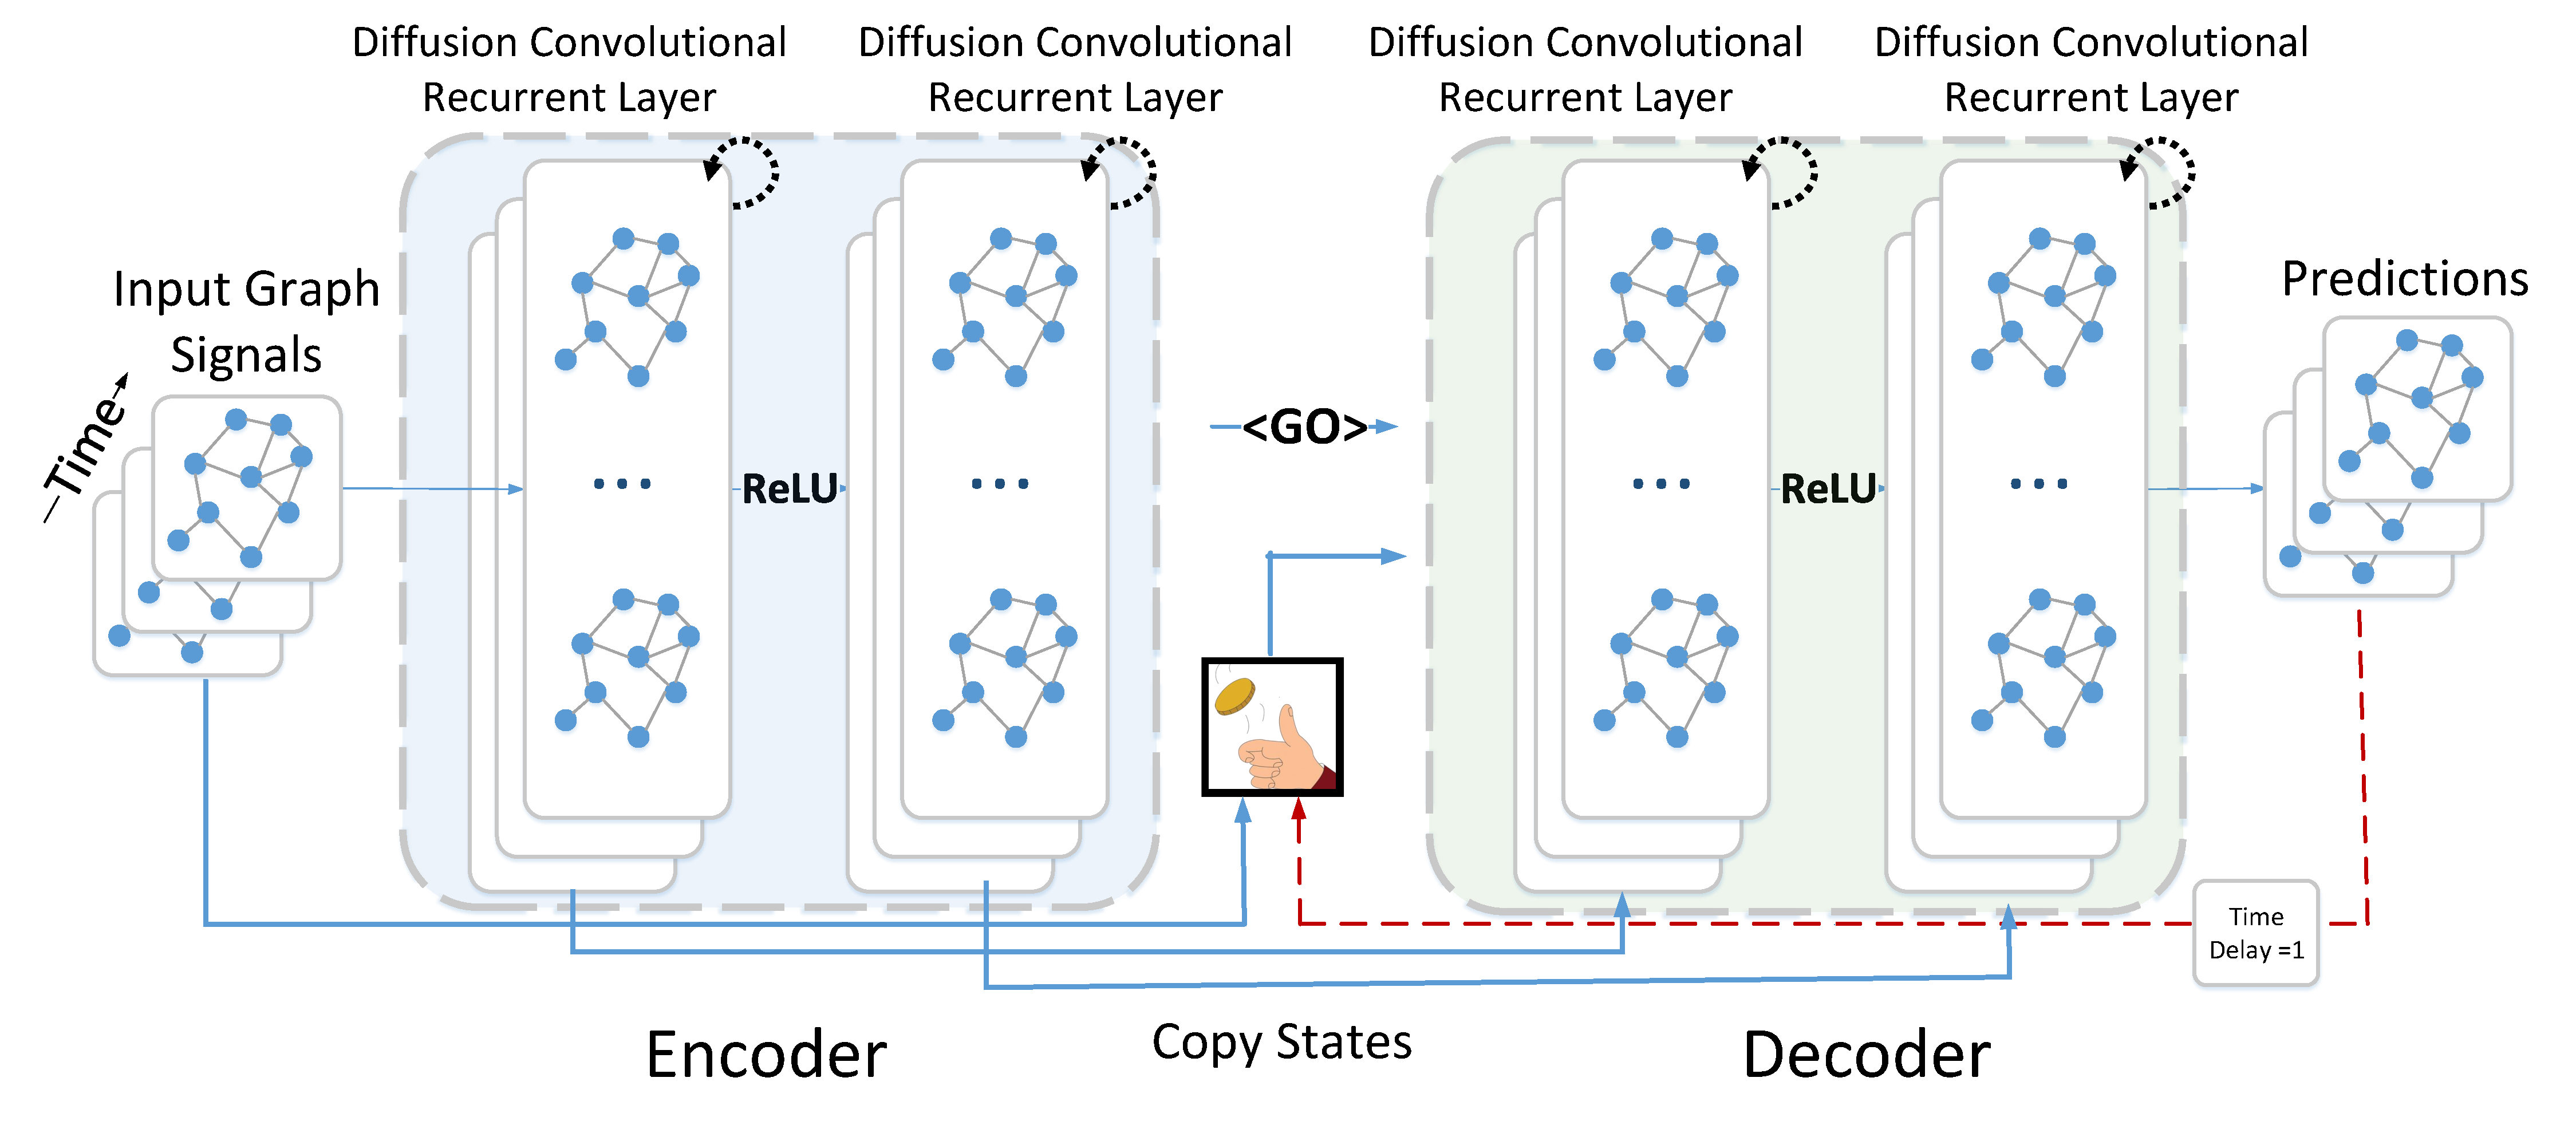
\includegraphics[width=\textwidth]{images/dcrnn_model_architecture.jpeg}
	\caption{DCRNN Model Architecture \cite{li2018dcrnn_traffic}}
	\label{fig:dcrnn-architecture}
\end{figure}

\subsubsection{Deep Seq2Seq Model}

Seq2Seq is a deep learning model used in time series forecasting for sequential information. It works by mapping an input sequence to a fixed-sized vector (i.e. hidden state) with an encoder and the hidden state to the target sequence with a decoder. The type of model explored for the encoder and decoder is the long short-term memory (LSTM) network \cite{hochreiter1997lstm}, which is designed for problems with long-term dependencies by addressing the vanishing gradient issue often encountered during model training \cite{huang2020aortic}. The general Seq2Seq architecture is displayed in Figure \ref{fig:seq2seq-architecture} below.

\begin{figure}[hbt!]
	\centering
	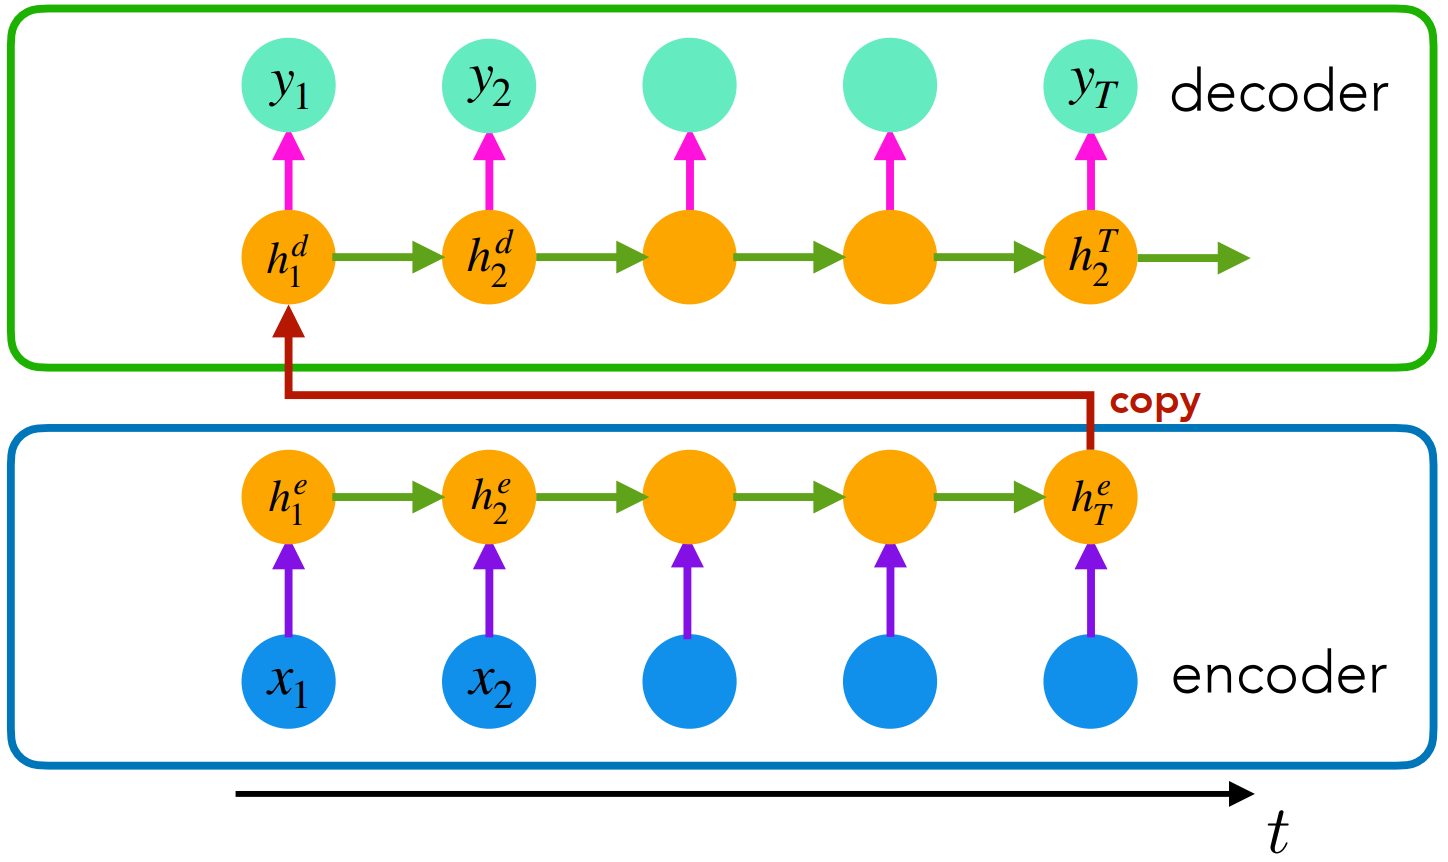
\includegraphics[width=0.8\textwidth]{images/seq2seq_architecture.png}
	\caption{Seq2Seq Model Architecture \cite{yu2021sequence}}
	\label{fig:seq2seq-architecture}
\end{figure}

\subsubsection{Classic Time Series Model}

The autoregressive neural network is a simple one-layer linear model where the model weights represent the coefficients of an autoregressive process. The implementation is influenced by the architecture of AR-Net \cite{triebe2019arnet}, which has been shown to correctly predict the true AR coefficients of a noisy AR process. What makes the model autoregressive is the input data representation. The time series to be modeled is transformed to a matrix where each row represents a model input and the number of columns is the lag or the order of the model, which also equals the number of input parameters in the linear layer. The target value is a future measurement at a desired forecasting horizon. The model is trained to minimize the mean squared error (MSE) of the total vehicle count, or the number of vehicles that cross a given traffic station over each five minute interval.

\begin{equation}
    X_t=c+\sum_{i=1}^{p} w_iX_{t-i}
\end{equation}

\subsubsection{Physics-Informed Neural Network}

The physics-informed neural networks implement numerical solutions to either ordinary differential equations (ODEs, used for COVID-19 modeling)
or partial differential equations (PDEs, used for the traffic model) relating functions and their derivatives.

\subsubsection{Prediction of COVID-19 cases using Physics-based Neural Network}
COVID-19 cases are predicted using a compartmental model
%The physics-informed neural network for the prediction of COVID-19 infections is based on a compartmental SEIR model 
\cite{zou2020epidemic} representing the size of the susceptible (S), exposed (E), currently infectious (I) and removed (R) population; the latter compartment includes both recovered and deceased patients. The SEIR model consists of a set of four coupled ODEs linking these populations using the time-dependent contact rate $\beta_t$, the recovery rate $\gamma_t$, and the incubation rate $\sigma_t$: 
\begin{align}
\frac{d S_t}{dt} &= - \frac{\beta_t I_t S_t}{N}, \\
\frac{d E_t}{dt} &= \frac{\beta_t I_t S_t}{N} - \sigma_t E_t \\
\frac{d I_t}{dt} &= \sigma_t E_t - \gamma_t I_t \\
\frac{d R_t}{dt} &= \gamma_t I_t
\end{align}

The four ODEs are solved numerically based on initial assumption of the model coefficients using an explicit Runge-Kutta (RK4) method. The model takes advantage of PyTorch’s auto-differentiation feature to carry out gradient descent using the Adam optimizer \cite{kingma2017adam}, and finds a set of model coefficients which explain the observations \cite{wang2020bridging}. The coefficients are allowed to vary over time, for example to capture changes in contact rates resulting from a stay-at-home ordinance. 

\subsubsection{Traffic prediction using the LWR model}
The physics-based neural network for traffic prediction uses the Lighthill-Whitham-Richards (LWR) model \cite{lighthill1955kinematic, richards1956shock}. It models traffic as a fluid stream and couples a partial differential equation representing conservation of mass with a fundamental equation relating traffic flow $q$, traffic density $k$ and 
traffic speed $u$:

\begin{align}
    \frac{\delta q}{\delta x} + & \frac{\delta k}{\delta t} = 0 \\
    q =& k v \\
    v =& v_f \frac{1-k}{k_j} \label{eq:greenshield}
\end{align}
where $x$ is the position along the road and $t$ denotes time.  
The parameters $k_j$ and $v_f$ represent the jam density and free-flow
velocity, respectively.
We use the Greenshield model \ref{eq:greenshield} as fundamental equation. The PDE in the LWR is solved numerically using an explicit finite difference scheme \cite{gaddam2016comparison}.  Again, we use PyTorch's auto-differentiation feature and the Adam optimizer to find the values of $k_j$ and $v_f$ which minimize the misfit between training data and predictions.  With these optimized parameters, traffic conditions (speed, density and flow) can be predicted into the future.

\section{Findings \& Reporting}

The models were trained to forecast average speed at 320 traffic station in the San Francisco Bay Area used in \cite{li2018dcrnn_traffic}. The original research used 325 stations, but 5 of those were not present in the data for the timeframe identified in 2020. Using the same sensors enabled us to leverage the existing adjacency matrix, whereas creating adjacency matrices for other geographic regions will require a robust method of identifying connectedness between traffic stations, i.e identifying the edges of the graph.

The models forecast speed at 5-minute intervals up to an hour in the future, but cannot exceed one hour without retraining with a longer horizon. The training data was selected from January through May 2020. The metric used to evaluate the predictions shown below is the mean absolute error (MAE). However, the models can use any regression loss function, such as root mean square error (RMSE) and mean absolute percentage error (MAPE). Figure \ref{fig:model-comparison} below shows a comparison of MAE for the different models across different horizons evaluated on data from June 2020. As expected, the DCRNN model outperforms both the Seq2Seq and autoregressive models since it models the spatial relationships between traffic sensors. However, it is curious that Seq2Seq is the worst-performing model and has decreasing error with increasing horizon. DCRNN and the autoregressive model both have the opposite trend, which makes intuitive sense. A forecasting model will naturally perform worse the further out in time it attempts to predict.

\begin{figure}[hbt!]
	\centering
	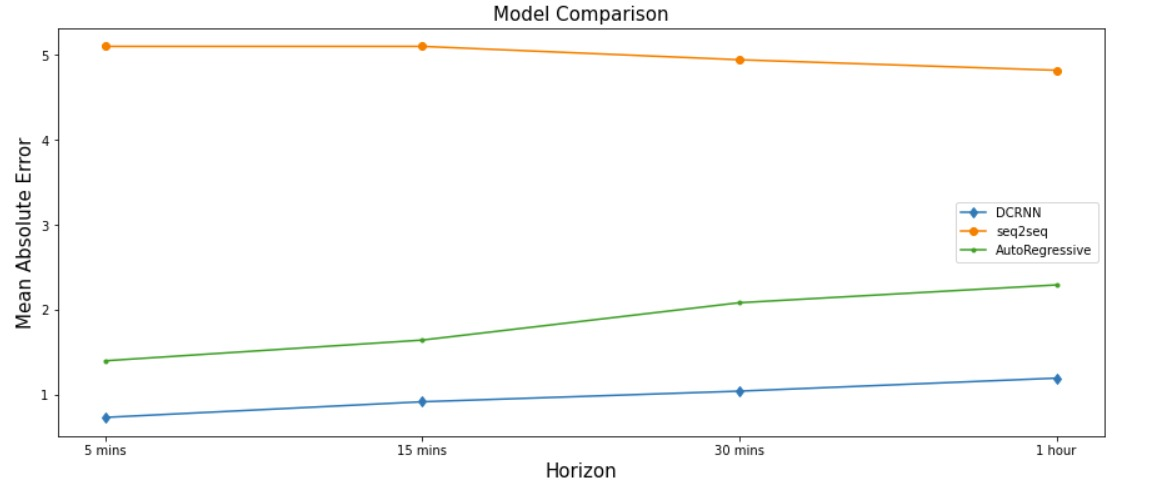
\includegraphics[width=0.8\textwidth]{images/model_comparison.jpeg}
	\caption{Traffic forecasting model comparison.}
	\label{fig:model-comparison}
\end{figure}

\subsection{General Traffic Forecasts}

The user can color a map in a desired location by traffic speed just like the traffic layer on Google Maps, but the forecasts are based on current data (assuming the model is being fed live data) rather than historical averages. Figure \ref{fig:traffic-forecast-map} below shows a map of San Diego with freeways colored by traffic speed, which provides a high-level view of the forecasted traffic an hour ahead of the input data. Traffic speeds are binned into four categories (depicting fast, moderate, slow, and very slow speeds) and colored accordingly. A categorical encoding is used instead of a continuous color scheme because small variations are not particularly helpful to the average user. The target audience for these predictions is the general public. The product could serve as an alternative to Google Maps and similar services for those interested in accurate forecasts and not just the current traffic. Since Google Maps is ubiquitous among route planning applications, selecting a similar presentation provides a familiar interface and makes it intuitive for new users. 

\begin{figure}[hbt!]
	\centering
	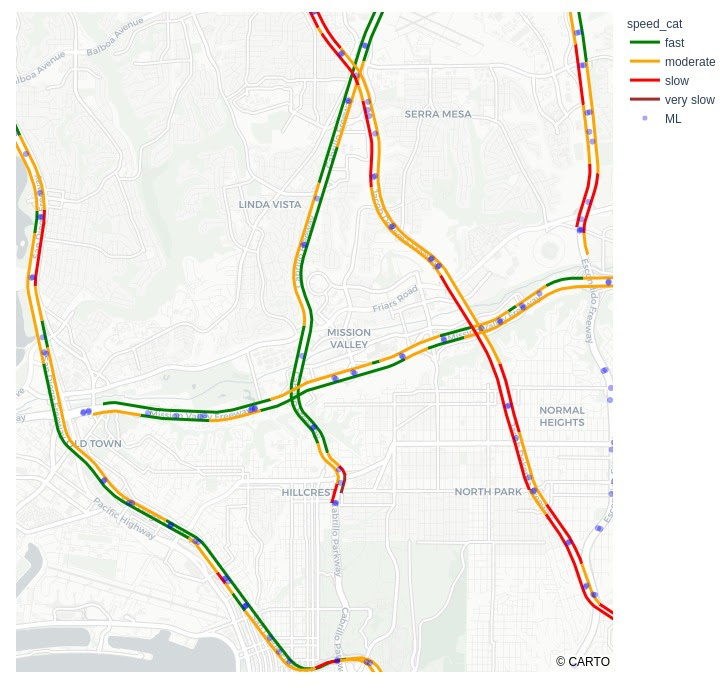
\includegraphics[width=0.75\textwidth]{images/traffic_map.jpeg}
	\caption{Traffic forecast}
	\label{fig:traffic-forecast-map}
\end{figure}

\subsection{Detailed Traffic Forecasts}

In addition to the map view described above, detailed traffic forecasts consist of speed predictions at 5-minute intervals presented as time series plots. The user is presented with a map similar to that in Figure \ref{fig:traffic-forecast-map}. Each dot on the map represents a traffic station in the Caltrans PeMS data. Clicking on a given point brings up a time series plot with the measured and predicted traffic speeds at the selected station over the desired timeframe and horizon, which can be up to an hour with the current model. This enables the user to narrow in on a particular location and get a detailed view of how the model is performing. Figure \ref{fig:traffic-time-series} below displays an example of a time series plot that will appear when the user selects a traffic station.

% An example of the traffic sensor network for the San Francisco Bay Area is shown below in Figure \ref{fig:bay-sensor-network}. Each sensor location is colored by freeway number.

% \begin{figure}[hbt!]
% 	\centering
% 	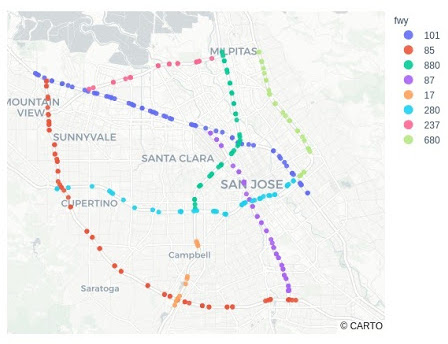
\includegraphics[scale=0.75]{images/bay_traffic_network.jpeg}
% 	\caption{Bay Area PeMS sensor network}
% 	\label{fig:bay-sensor-network}
% \end{figure}

\begin{figure}[hbt!]
	\centering
	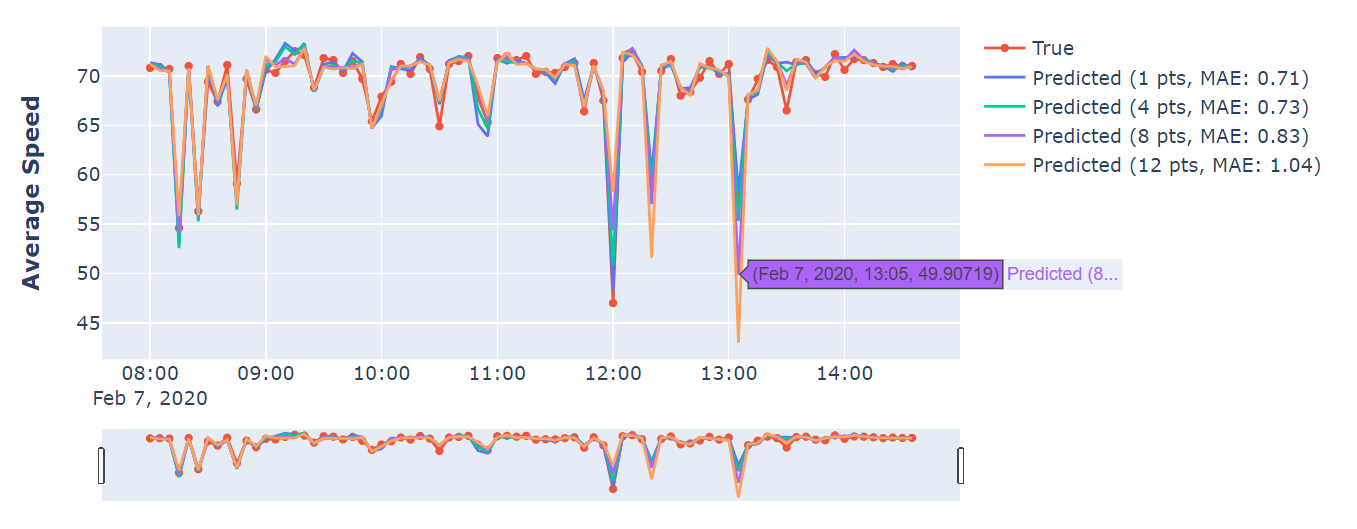
\includegraphics[width=\textwidth]{images/traffic_time_series.png}
	\caption{Traffic forecast at a single station.}
	\label{fig:traffic-time-series}
\end{figure}

The user can also change the map view to color freeways by model prediction error (shown below in Figure \ref{fig:traffic-error-map}). This allows the user to identify any geographic regions where the model is underperforming relative to the rest of the network and thus requires further investigation.

\begin{figure}[hbt!]
	\centering
	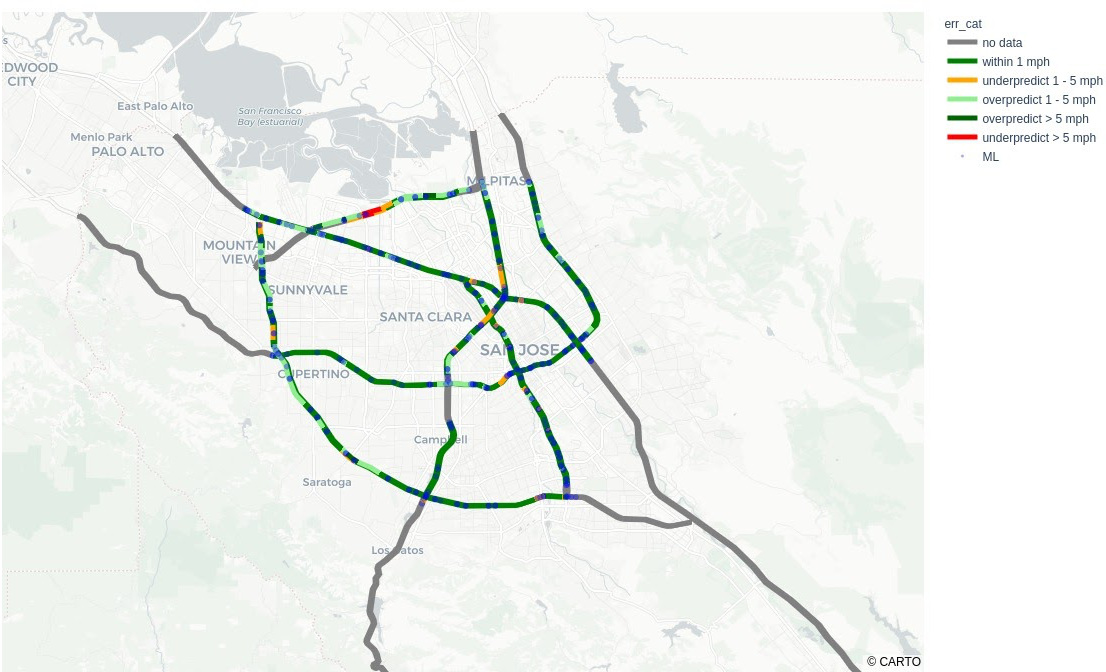
\includegraphics[width=0.75\textwidth]{images/traffic_map_error.jpeg}
	\caption{Traffic forecast error}
	\label{fig:traffic-error-map}
\end{figure}

The audience for the detailed traffic forecasts are traffic engineers at Caltrans or other data scientists working on traffic-related projects. Since traffic data is spatiotemporal in nature, providing snapshot information on a map and stationary information as time series plots is a natural presentation. The dashboard was designed based on correspondence with a traffic engineer at Caltrans.

\subsection{Traffic Forecasts using LWR Model}

The LWR model for macroscopic traffic prediction was trained on 5 hours of data collected by receivers along southbound I5 between San Onofre and Encinitas on November 11, 2019.  We then used to optimized model parameters (jam density $k_j$ and free velocity $v_f$) to predict conditions 5 and 10 minutes into the future. Predicted velocities are typically close to 30 m/s (67 miles per hour), except at the end of the segment close to N/O Vista View ramp where they drop to 25 m/s 
consistent with the true velocities (Fig.~\ref{fig:lwr}).

\begin{figure}[hbt!]
    \centering
    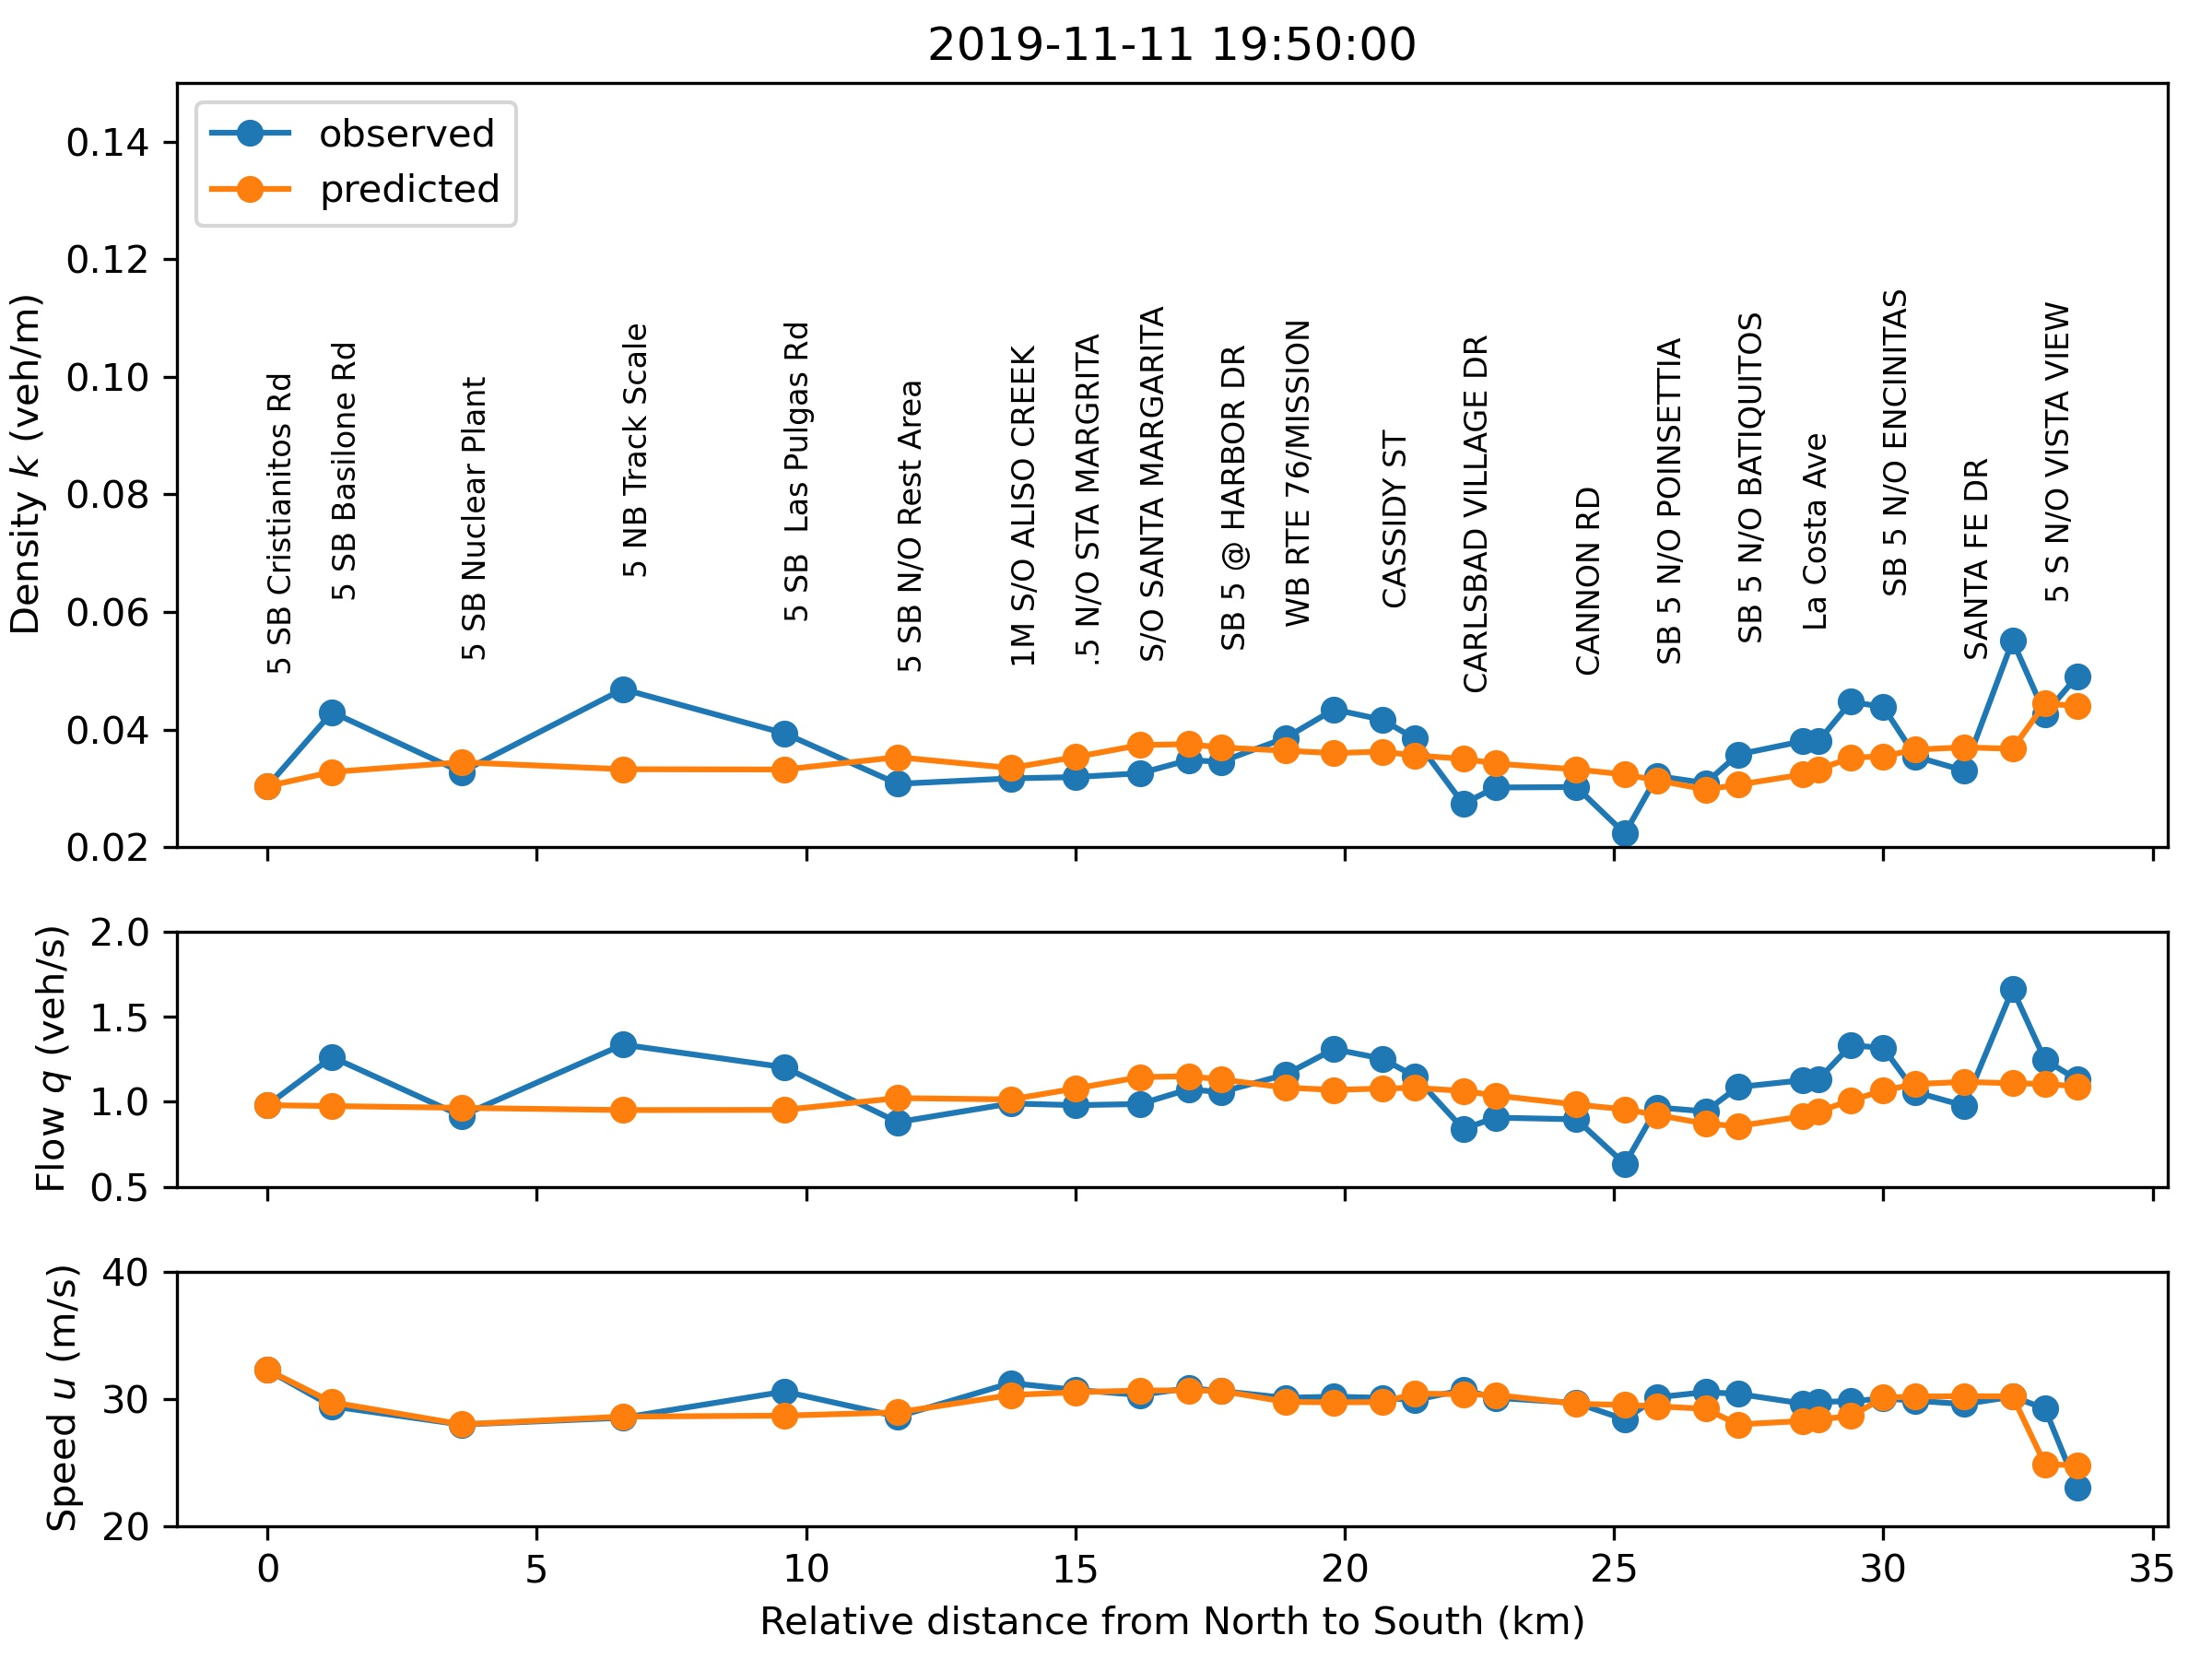
\includegraphics[width=\textwidth]{images/LWR_prediction_5S.jpg}
    \caption{Predictions of traffic density $k$, flow $k$ and average velocity $u$ as function of distance along southbound I-5 obtained from LWR model compared to true traffic.}
    \label{fig:lwr}
\end{figure}

\subsection{COVID-19}

In addition to forecasting traffic, the physics-informed neural network methodology was also used to predict the number of new COVID-19 cases as a test case. Forecasting the number of infected and death from COVID-19 using deep learning is particularly challenging due to shifted distributions in both the data and parameter domain \cite{wang2020bridging}.

The compartmental model was trained on COVID-19 data from San Diego County spanning the period from January 22, 2020 to January 29, 2021 (373 days); and predictions were made for the two weeks from January 30 to February 12, 2021.  As the Johns Hopkins dataset only includes cumulative cases, we estimated the size of the currently infectious population (Fig. \ref{fig:seir}) based on a recovery period of 14 days \cite{lange2021covid}.  The network was trained for a total of 300 epochs; and the MSE converged to a value below 2.5$\cdot$10$^{-7}$.

 \begin{figure}[hbt!]
     \centering
     \begin{subfigure}[b]{0.48\textwidth}
         \centering
         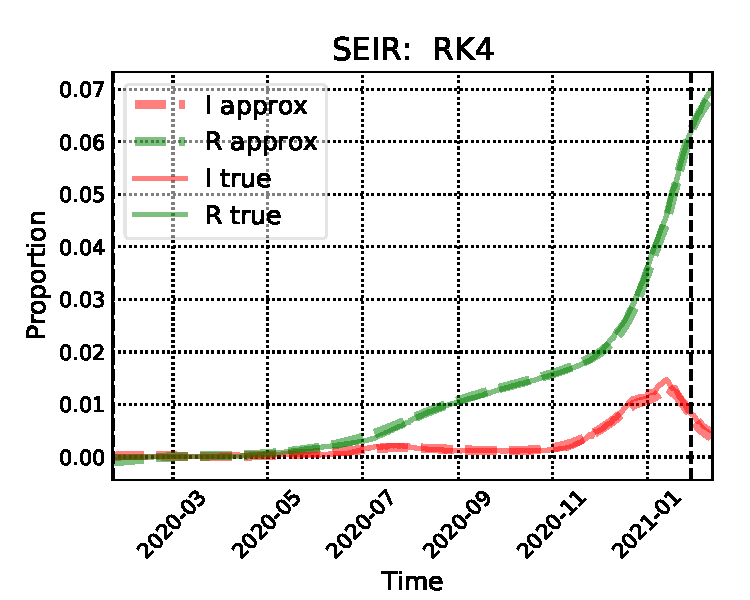
\includegraphics[width=\textwidth]{images/seir_pde_const_sigma_prop.pdf}
         \caption{Normalized size of observed and predicted currently infected (I) and removed (R) populations.}
         \label{fig:seir1}
     \end{subfigure}
     \hfill
     \begin{subfigure}[b]{0.48\textwidth}
         \centering
         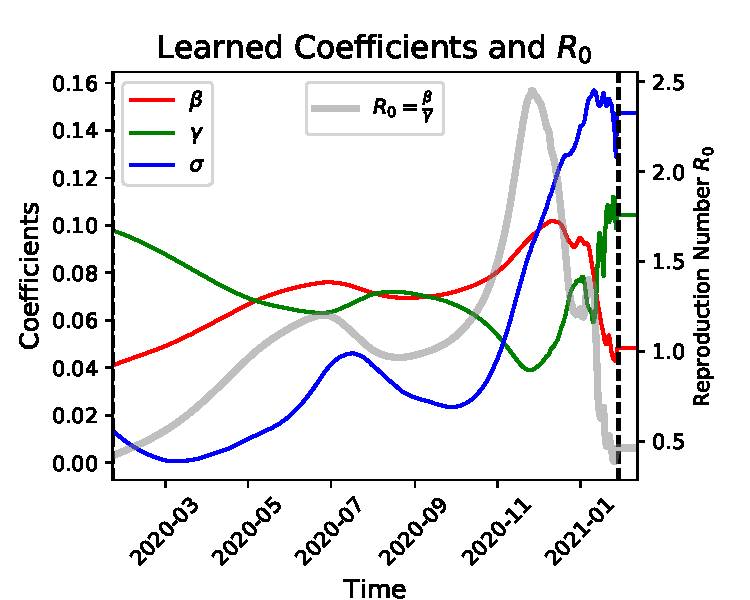
\includegraphics[width=\textwidth]{images/seir_pde_const_sigma_param.pdf}  
         \caption{Model coefficients and basic reproduction number $R_0$ as a function of time. }
         \label{fig:seir2}
     \end{subfigure}
     \caption{COVID-19 prediction using SEIR model.  Dashed lines represent the end of the training window.}
     \label{fig:seir}
 \end{figure}

%\begin{figure}[hbt!]
%\begin{center}
%\includegraphics[width=\textwidth]{images/SEIR_timedep_const_sigma.pdf}
%\caption{\emph{(a)} Normalized size of observed and predicted currently infected (I) and removed (R) populations from physics-based COVID-19 model.  \emph{(b)} SEIR model coefficients and basic reproduction number $R_0$ as a function of time. Dashed lines represent the end of the training window.}
%\label{fig:seir}
%\end{center}
%\end{figure}

The progression of the currently infected population (Fig.~\ref{fig:seir}) shows two peaks, reflecting the two waves of the pandemic recorded in July and December 2020, respectively.  
The simulated size of the currently infected and removed population reproduces these features during the training window, and correctly extrapolates the development two weeks into the future.  
Learned coefficients indicate elevated contact rates in July and December 2020.  The basic reproduction number, calculated as $R_0 = \frac{\beta}{\gamma}$ \cite{zou2020epidemic}
exceeded a value of 2.0 during the holiday season 2020, but dropped dramatically in subsequent weeks.

\subsection{Dashboard}

The map view of forecasted traffic was implemented in Mapbox\footnote{\url{https://www.mapbox.com/}} using Plotly\footnote{\url{https://plotly.com/}} and Python, while the web interface to the map was developed using Dash. The forecasted traffic is visualized using color-coded lines plotted on top of a background map (Figure \ref{fig:sensor-density-fine}), where the color code reflects a category of mean vehicle speed (fast, medium, slow, stopped). Because the relatively sparse density of PeMS sensors does not result in a visually appealing road representation if sensors are connected through straight segments (Figure \ref{fig:sensor-density-coarse}), we augmented the visualization using more accurate road location data (Figure \ref{fig:sensor-density-fine}) from USDOT. The original PeMS traffic stations are displayed as the points on the map. Road coordinates were extracted for each freeway and direction covered by PeMS sensors, and absolute position markers were computed for each USDOT data point. These higher-resolution road representations were added to the AWS RDS database. Using finer-resolution data allows the user to easily distinguish between the two directions of each freeway, which is infeasible with the coarse PeMS data. In addition, freeways in the traffic visualization augmented with USDOT data align nicely with freeways in the background map.

\begin{figure}[hbt!]
    \centering
    \begin{subfigure}[b]{0.48\textwidth}
        \centering
        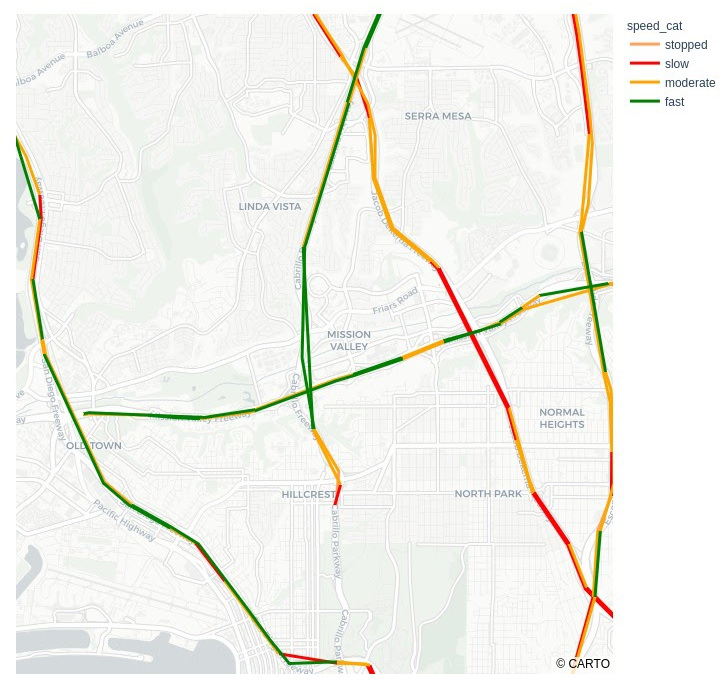
\includegraphics[width=\textwidth]{images/traffic_map_coarse.jpeg}
        \caption{Original PeMS stations}
        \label{fig:sensor-density-coarse}
    \end{subfigure}
    \hfill
    \begin{subfigure}[b]{0.48\textwidth}
        \centering
        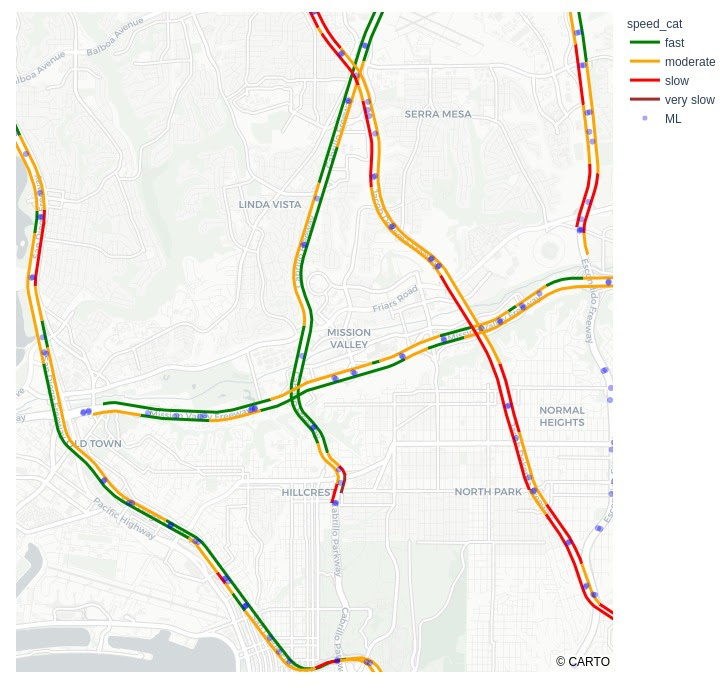
\includegraphics[width=\textwidth]{images/traffic_map.jpeg}
        \caption{Higher-resolution USDOT freeway coordinates}
        \label{fig:sensor-density-fine}
    \end{subfigure}
    \caption{Comparison of traffic maps with different spatial densities.}
    \label{fig:sensor-density-comparison}
\end{figure}

The reporting dashboard, shown below in Figure \ref{fig:dashboard}, is built using Python Plotly and Dash packages to create each of the visualization elements and app interactivity. Many of the visuals included in the layout are controlled with core components, such as filters and dropdown menus, to not only give the user the ability to focus on a particular subset of the data, but also to provide rendering optimizations. For framed visualizations, such as showing data from a time series range, a play button is available for some views in order to easily scan through the data or to hone into a specific time period. Lastly, every element with Dash is highly interactive in order to provide the user tools for detailed analysis such as hovering metadata popup window, in/out zoom, and downloading a snapshot for the visualization.

\begin{figure}[hbt!]
	\centering
	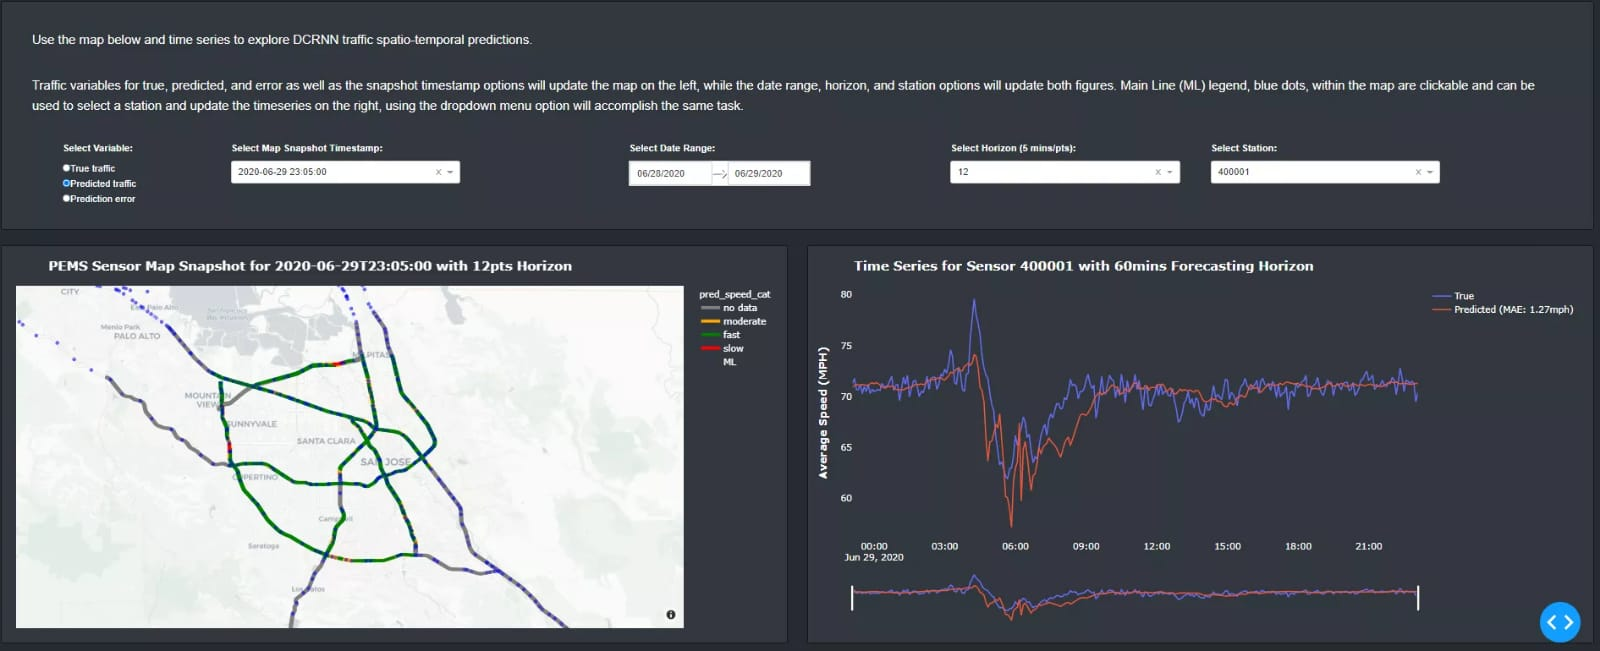
\includegraphics[width=\textwidth]{images/dashboard.jpeg}
	\caption{Traffic Dashboard}
	\label{fig:dashboard}
\end{figure}

The reporting dashboard aims to provide storytelling via exploratory data analysis for both the traffic and COVID-19 datasets. It then integrates channels to visualize time series predictions for the DCRNN model trained to support a predictive horizon from 5 minutes up to 1 hour (as shown in Figure \ref{fig:dashboard} above).

The exploratory data analysis views include following:
\begin{itemize}
    \item View which shows average speed (averaged over 5-minute window) over the course of an average day for the same time frames. It conveys a higher variation in speed due to more traffic during rush hours for months before the COVID-19 pandemic.
    \item View to analyze the traffic speed with respect to new COVID-19 cases by calendar days in 2020.
    \item Pearson correlation matrix comparing COVID-19 and Caltrans traffic dataset.
\end{itemize}

The DCRNN traffic model prediction visuals include:
\begin{itemize}
    \item Single-select options for station number and prediction horizons. 
    \item Date range and range slider for narrowing the time series axis. 
    \item A view with line charts for true and predicted ``average speed'' values for the selected horizon, where the MAE is included in the legend.
\end{itemize}

\section{Solution Architecture, Performance \& Evaluation}

\subsection{Compute Resources}

The compute architecture consists of a PostgreSQL database hosted on Amazon RDS and an Amazon Elastic Compute Cloud (EC2)\footnote{\url{https://aws.amazon.com/ec2/}} instance for model training and inference. The initial EC2 instance threshold was insufficient to train the DCRNN model. Once the threshold was increased to 32 vCPUs, the larger g4dn.4xlarge and p2.8xlarge instances became available, which proved sufficient to train the DCRNN model. A free alternative to EC2 is Nautilus,\footnote{\url{https://nautilus.optiputer.net/}} which is a Kubernetes cluster for running containerized big data applications.\footnote{\url{https://ucsd-prp.gitlab.io/nautilus/}} Nautilus is part of the Pacific Research Platform (PRP), a partnership led by researchers from UC San Diego and UC Berkeley. The p2.8xlarge EC2 instance costs \$7.20/hr, which can quickly add up. However, Nautilus is a shared resource and the necessary GPUs are not always available. We ultimately used a combination of EC2 and Nautilus to train the models.

Amazon S3, RDS, and small EC2 instances incur very little cost. The primary expense for the team was from the large EC2 instances, namely the g4dn.4xlarge and p2.8xlarge instances mentioned above. When we were requesting increases to the EC2 thresholds, we calculated the amount of compute time we could utilize based on the expenses of the the AWS services we were running. Fortunately, the UCSD AWS accounts provide spending reports upon login, providing a clear view of what services are being charged and our remaining budget.

\subsection{Scalability \& Robustness}

The PeMS and Johns Hopkins data sources generate data on a daily basis. While the Johns Hopkins dataset is fairly small at under 100 MB, PeMS generates about 120 MB of data per day for the entirety of California. Further, since our DCRNN model is dynamic, that is we perform operations on traffic networks, the network sizes vary pretty frequently in the real world. Our model must be scalable in terms of data, which is that the model should be able to train and continue to perform well in terms of MAE or MSE scores even as the data scales. Furthermore, the model should be scalable in terms of graph nodes as well, meaning that DCRNN should be scalable to a large network of sensors. This might need us to think about memory and compute constraints. Also, the model should be robust along differences in network architectures caused by hyperparameter tuning. Some architectures might cause the number of parameters to grow significantly and the implementation should be robust enough to handle such tuning. Thus a model that generalizes well to the increasing amount of data in both the temporal and spatial dimensions and generates at least the same amount of mean errors if not better could be considered as a scalable one.

The scalability analysis was divided into multiple different tasks. First the scalability of the database is ensured by upgrading database performance, such as by creating indices and upgrading the AWS instance type. Further, materialized views were created where data access was frequent or logically separate from the data ingestion. This helped access data efficiently and also make sure data was refreshed only when required. The scalability of the model was divided into data, model, and compute scalability to address all the challenges that could arise in a real world application. Data scalability aims at testing how the model performs with an inflow of more data. For data scalability we test not only the number of rows, but also the addition of extra nodes to the network of traffic sensors. For model scalability we make sure to test different model architectures by means of tuning parameters such as the number of stacked recurrent neural network (RNN) layers and the number of diffusion steps in the diffusion process. This approach ensures a definite change in the number of parameters of the model and gives us an idea of how well the model scales. Finally compute scalability aims at testing how well the model scales with compute resources. This was performed by creating a robust implementation of DCRNN using PyTorch Lightning\footnote{\url{https://www.pytorchlightning.ai/}} that allowed us to implement parallelism on multiple GPUs. The approach tests parallelism across 1 node, however the same implementation should work for distributed data parallelism if the need arises.

We use a masked mean absolute error for the evaluation of DCRNN speed predictions. The strategy of evaluation differs for each scalability test. For data pipeline scalability, data access speed is the metric used to test how well the data pipeline will scale. For data scalability of the model, we make sure that the model can effectively learn from different volumes of data. For model scalability, we make sure each network architecture yields an MAE that corresponds to the nature of the network, meaning that each network architecture change does what it is expected to do. A secondary check is to ensure that modifying a hyperparameter does not result in dramatically increased training times. For compute scalability, the strategy is to make sure the loss convergence is similar to that of the previous implementation and to make sure training time reduces with the availability of more compute resources.

To evaluate spatiotemporal predictions for scalability and robustness, the DCRNN model was evaluated in three main areas of interest: model, dataset, and compute. In other words, the algorithm is tested to characterize its ability to handle changing model parameters, varying or increasing amounts of data, and single to multiple computational resources. Some of the requirements are not only that it has to effectively learn under these controlled test cases, but it also has to be able to predict with consistent train and testing errors under reasonable time and resources.

\subsubsection{Database Robustness}

The Postgres database instance hosted on AWS-RDS was adjusted and tuned to optimize data retrieval for training and validation of time series models. Due to the small size of the COVID-19 data source, which represented no challenges, these efforts focused on the traffic data. Prior to these optimizations, a query for traffic data collected within one calendar month (e.g., \char`\~13 million tuples for San Diego county data collected in January 2021) took roughly 15 minutes to return. Creating an index on the date of the timestamp (not represented in a dedicated column) reduced the query time to just two minutes. In addition, the database service was transferred from a t2.micro to a m6g.large instance for better performance.

\subsubsection{Data Scalability}

DCRNN model performance with varying dataset sizes is evaluated by incorporating different numbers of nodes into the network graph including 80, 160, and 240 nodes, which represent a sub-sample of 25\%, 50\%, and 75\% respectively from the current total number of nodes of 320. The network starts with the smaller subset of nodes and is then expanded outwards by including neighboring stations. Using this approach the model can be evaluated for scalability as the number of stations increases, similarly as more freeways and roads are added in the city network surroundings.

When comparing model performance, the loss shown in Table \ref{tab:data-scale} below shows that error increases proportionally with the number of nodes. However, this observation does not hold when the subset of the graph is compared as more nodes are added to the model. For example, the MAE for 25\% of the nodes goes down when the model is trained with 50\% of the nodes from 0.8697 to 0.8644. It decreases even further to 0.8638 when 75\% of the nodes are used. In short, this study shows how the model is able to handle increased data size by comparing MAE when incorporating additional spatial components and also brings up the observation that existing node predictions are improved with the addition of this information. Additionally, the compute time per epoch seems to scale reasonably well with the increasing number of nodes as shown in Table \ref{tab:data-scale} below. The models using subsets of the full graph were trained on a NVIDIA GeForce GTX 1080 GPU. However, the 1080 only has 8 GB of memory, which is insufficient to train the DCRNN model on the full 320-node graph. Therefore, the model with the full graph was trained on a NVIDIA GeForce RTX 2080 Ti GPU, which has 11 GB of memory. To account for the performance difference between the 1080 and 2080 Ti, the average time per epoch calculated with the 2080 Ti was scaled by 160\%\footnote{https://www.techpowerup.com/gpu-specs/geforce-gtx-1080.c2839} as a rough estimate for the epoch time if the full DCRNN model were trained on a 1080 GPU.

\begin{table}[hbt!]
	\caption{DCRNN Data Scalability Study}
	\centering
	\begin{tabular}{ccr}
		\toprule
		Graph Size                  & Avg. Epoch Time (s)   & MAE \\
		\midrule
		80 (25\%)                   & 574                   & All: 0.8697 \\
		\midrule
		\multirow{2}{*}{160 (50\%)} & \multirow{2}{*}{764}  & All: 0.9087 \\ & & 25\%: 0.8644 \\
		\midrule
		\multirow{3}{*}{240 (75\%)} & \multirow{3}{*}{1015} & All: 0.9667 \\ & & 50\%: 0.9033 \\ & & 25\%: 0.8638 \\
		\midrule
		\multirow{4}{*}{320}        & \multirow{4}{*}{1432\textsuperscript{\textasteriskcentered}}    & All: 1.0251 \\ & & 75\%: 0.9893 \\ & & 50\%: 0.9792 \\ & & 25\%: 0.9428 \\
		\bottomrule \\
		\multicolumn{2}{l}{\textsuperscript{\textasteriskcentered}Original value scaled by 1.6}
	\end{tabular}
	\label{tab:data-scale}
\end{table}

\subsubsection{Model Scalability}

Model scalability is tested by assessing the compute time for different network architectures, which in turn is accomplished by controlling a series of hyperparameters. The hyperparameters that determine the total number of DCRNN model parameters are the number of diffusion convolutional gated recurrent unit (DCGRU) layers, the number of units within each DCGRU layer, and the number of diffusion steps in each layer. The baseline model is composed of 2 layers with 64 units, each using 2 diffusion steps. A summary of the various models trained is provided below in Table \ref{tab:model-scale}. The parameter sweeps are performed by modifying each parameter in isolation from the baseline configuration. For example, the network with 3 DCGRU layers contains 64 RNN units with 2 diffusion steps. The intent is not to provide an exhaustive search, but rather to explore how the DCRNN training time generally scales with the number of parameters.

\begin{table}[hbt!]
	\caption{DCRNN Model Scalability Study}
	\centering
	\begin{tabular}{ccccc}
		\toprule
% 		\multicolumn{2}{c}{Part}                   \\
% 		\cmidrule(r){1-2}
		Layers   & RNN Units & Diffusion Steps & Model Parameters (x1000)   & Avg. Epoch Time (s) \\
		\midrule
		1        & 64        & 2               & 126.2                      & 504 \\
		2        & 32        & 2               & 94.0                       & 707 \\
		2        & 64        & 1               & 223.7                      & 713 \\
		2        & 64        & 2               & 372.4                      & 1371 \\
		2        & 64        & 3               & 521.0                      & 2038 \\
		2        & 96        & 2               & 835.0                      & 2067 \\
		3        & 64        & 2               & 618.5                      & 2213 \\
		\bottomrule
	\end{tabular}
	\label{tab:model-scale}
\end{table}

Given that the purpose of this study is to evaluate model scalability and not perform hyperparameter tuning, each model is only trained for 5 epochs. Five epochs is insufficient to train the DCRNN model, but it provides a reasonable estimate of the training time since the time per epoch is relatively constant. Each model is trained on an AWS EC2 g4dn.4xlarge instance, which provides an NVIDIA Tesla T4 GPU with 16 GB of memory. The batch size of each model was set to the highest power of two that would fit within memory, which ranged from 64 to 256. Figure \ref{fig:model-scale-split} below displays the results of each parameter sweep. All exhibit remarkably linear growth in training time with respect to the parameter being varied. Varying the number of layers provides the largest difference in training time, ranging from roughly 500 seconds per epoch with one layer to 2250 seconds per epoch with three layers.

\begin{figure}[hbt!]
	\centering
	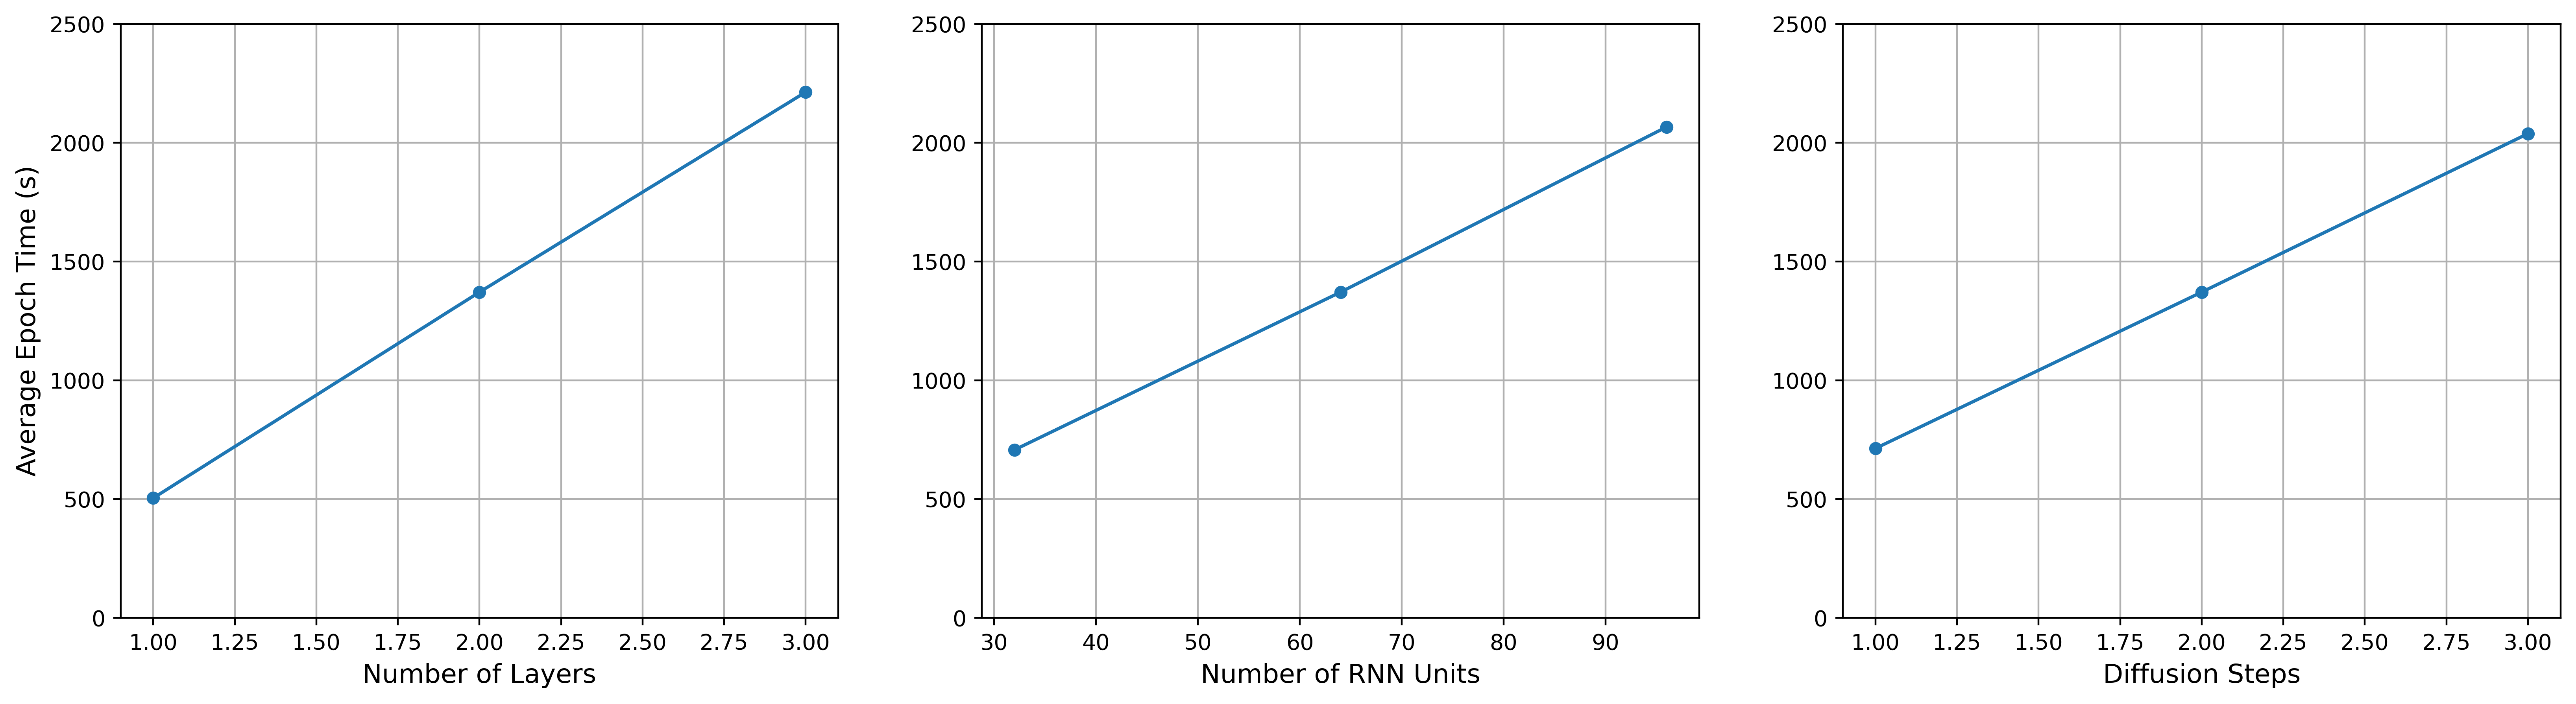
\includegraphics[width=\textwidth]{images/model_scale_split.png}
	\caption{DCRNN epoch times for individual hyperparameter sweeps.}
	\label{fig:model-scale-split}
\end{figure}

Figure \ref{fig:model-scale} conveys the same information relative to the number of model parameters. The number of parameters ranges from roughly 100,000 to 850,000 for the network architectures tested. The range in epoch times between the RNN unit and diffusion step sweeps are nearly identical, despite the fact that the range in the number of parameters for the RNN unit sweep is nearly 2.5 times that of the diffusion step sweep. This is potentially caused by the nature of how each hyperparameter is implemented. Increasing the number of diffusion steps, as well as the number of layers, increases the number of loops iterations in the model. However, increasing the number of RNN units increases the size of the matrix multiplication performed in each layer, which is more efficient than increasing the number of iterations in loops.

\begin{figure}[hbt!]
	\centering
	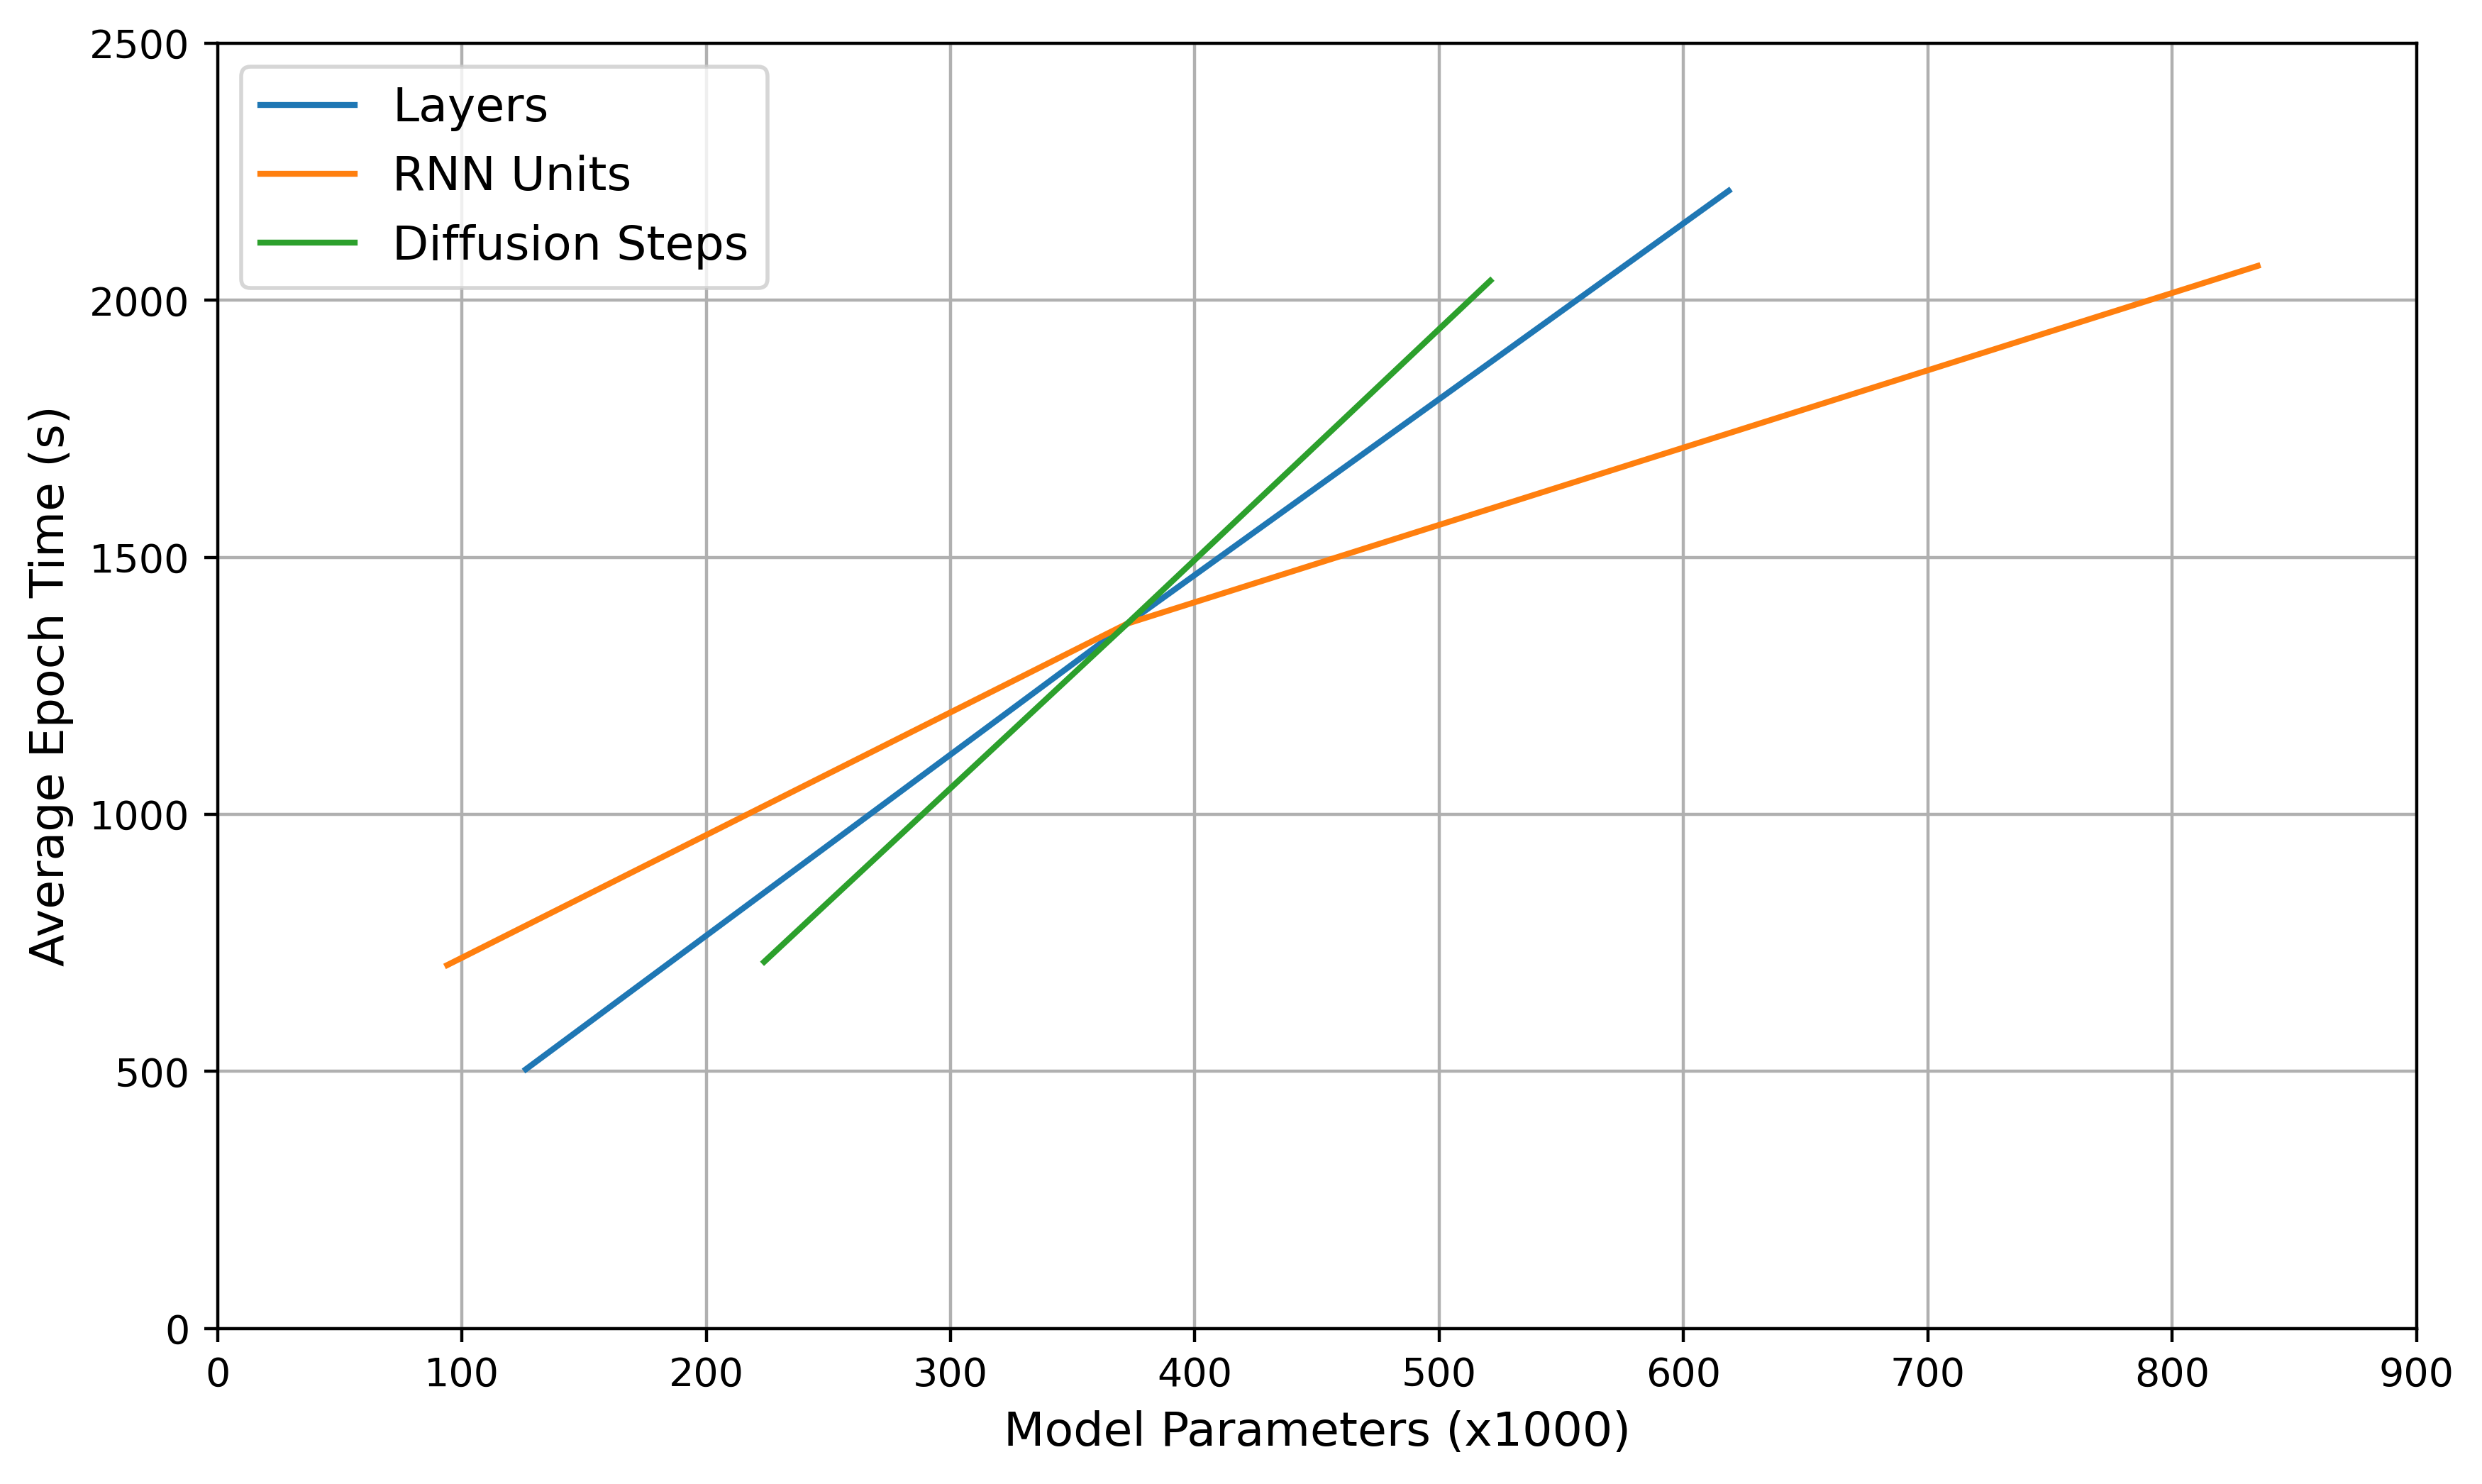
\includegraphics[scale=0.65]{images/model_scale.png}
	\caption{DCRNN epoch times for different model configurations.}
	\label{fig:model-scale}
\end{figure}

\subsubsection{Compute Scalability}

The original implementation of DCRNN was meant to be executed on 1 GPU, and was not designed for compute scalability. In order to abstract the existing implementation and also enable compute scalability, the existing code was wrapped around PyTorch Lightning. Such an implementation has allowed us to scale to multiple GPUs with minimal code change and also choose between a data parallel (DP) scalability approach and a distributed data parallel (DDP) approach, irrespective of what infrastructure is underneath.

Using p2.8xlarge instances (upto 8 NVIDIA K80 GPUs) on AWS and the PyTorch Lightning implementation of DCRNN allowed us to scale to upto 8 GPUs. Below in Table \ref{tab:compute-scale} we can see results of experiments where we increase the number of GPUs given to our model, and receive improved compute times per epoch.

\begin{table}[hbt!]
	\caption{DCRNN Compute Scalability Study}
	\centering
	\begin{tabular}{cc}
		\toprule
		Number of GPUs  & Avg. Epoch Time (s) \\
		\midrule
		1               & 6182 \\
		2               & 1516 \\
		4               & 794 \\
		6               & 442 \\
		8               & 248 \\
		\bottomrule
	\end{tabular}
	\label{tab:compute-scale}
\end{table}

The table illustrates a considerable amount of scaling. The scaling factor is quite large from 1 GPU to 2 GPUs (\char`\~4). However, there are diminishing returns and the improvement decreases when increasing the number of GPUs from 4 to 8 (\char`\~3). This helps us infer that adding more GPUs only helps up until a point and later proves to add overhead. 

This scaling however does come at a cost. DCRNN’s adjacency matrix was originally intended to be a sparse tensor implementation, which makes sense because most of the edges in a graph are not connected and the adjacency matrix would end up with many zeros and thus occupy more memory than required. However, PyTorch concurrency features fail to work with sparse features and force us to implement DCRNN using dense adjacency matrix tensors. While this does help in compute time scaling, it does use more memory and causes us to reduce the batch size. This gives us an area to work on and improvise in the future, since we would have to come up with a solution that generalizes well.

\section{Conclusions}

There are many factors that influence daily traffic patterns, including road work, traffic accidents, large sporting events, or as was the case in 2020, a global pandemic.
Traffic models that have been calibrated on historical data recorded before the pandemic may not fully capture the disruptions in traffic patterns caused by remote work and changed consumer behavior.
In order to better capture day-to-day traffic variations,
we have explored several dynamic machine learning models, including a classic time series model,
a seq2seq model, a diffusion convolutional recurrent neural network (DCRNN), and a 
physics-informed neural network.
While this study focused on traffic patterns in San Diego county and in the Bay area, our conclusions are
likely valid outside of these regions.

We have developed a data processing pipeline to retrieve and extract information on freeway traffic from PEMS sensors, 
detailed representations of the freeway network from USDOT, and daily Covid-19 case numbers from John Hopkins University.
A relational database was deployed to host these records, and the scalability and robustness of the
database was fine-tuned to allow quick retrieval of training and testing data for model re-calibration.
Exploratory analysis of traffic patterns and Covid-19 cases confirmed that the onset of the pandemic was accompanied
by a drastic reduction in rush hour traffic, reflected by reduced vehicle counts and improved average vehicle velocity
during the pandemic's onset with respect to a pre-pandemic reference timeframe.
Although our experiments with the four different time-series forecasting models show that all methods have their strengths
in the prediction of traffic patterns and Covid-19 cases, the DCRNN  emerged 
%we settled for the DCRNN 
as our minimum viable modeling product as it accurately predicts short-term variations in road traffic across the freeway 
network.

A reporting dashboard was deployed which allows the user to explore spatial or temporal 
patterns in traffic predictions by interactively controlling a map and time series view.
User-controllable elements in the dashboard include the time and date, the prediction horizon, 
the variable displayed in the map view
(i.e., the predicted or true traffic or the prediction error), and the sensor shown in the time series view.

We made extensive use of several AWS resources including RDS for running a PostgreSQL server, regular and GPU-powered EC2 
instances for model training and inference, and S3 buckets for raw data storage.  
The Nautilus Kubernetes cluster was also used for some model training.

\printbibliography
% \bibliographystyle{unsrt}
% \bibliography{references}  %%% Uncomment this line and comment out the ``thebibliography'' section below to use the external .bib file (using bibtex) .


%%% Uncomment this section and comment out the \bibliography{references} line above to use inline references.
% \begin{thebibliography}{1}

% 	\bibitem{kour2014real}
% 	George Kour and Raid Saabne.
% 	\newblock Real-time segmentation of on-line handwritten arabic script.
% 	\newblock In {\em Frontiers in Handwriting Recognition (ICFHR), 2014 14th
% 			International Conference on}, pages 417--422. IEEE, 2014.

% 	\bibitem{kour2014fast}
% 	George Kour and Raid Saabne.
% 	\newblock Fast classification of handwritten on-line arabic characters.
% 	\newblock In {\em Soft Computing and Pattern Recognition (SoCPaR), 2014 6th
% 			International Conference of}, pages 312--318. IEEE, 2014.

% 	\bibitem{hadash2018estimate}
% 	Guy Hadash, Einat Kermany, Boaz Carmeli, Ofer Lavi, George Kour, and Alon
% 	Jacovi.
% 	\newblock Estimate and replace: A novel approach to integrating deep neural
% 	networks with existing applications.
% 	\newblock {\em arXiv preprint arXiv:1804.09028}, 2018.

% \end{thebibliography}

\begin{appendices}

\section{DSE MAS Knowledge Applied to the Project}

This project required applying knowledge and skills gained from the majority of classes in the UCSD DSE MAS program. The project made heavy use of Python programming, web scraping, data wrangling, relational databases, machine learning, and data visualization. The courses most heavily utilized in this project include:

\begin{itemize}
    \item Python for Data Analysis (DSE 200)
    \item Data Management Systems (DSE 201)
    \item Data Integration \& ETL (DSE 203)
	\item Machine Learning (DSE 220)
	\item Data Visualization (DSE 241)
\end{itemize}

\section{Link to UCSD Library Archive}

This project is archived at the UCSD Library Digital Collections\footnote{\url{https://doi.org/10.6075/J03F4PHC}} to ensure results are reproducible and ensure future projects can build upon this work. The archive includes the following:

\begin{itemize}
    \item PeMS traffic and Johns Hopkins COVID-19 data
    \item Source code used to collect data, train models, and create visualizations
    \item TorchTS library in its state at time of publication
    \item This report, presentation slides, and project poster
\end{itemize}

\end{appendices}

\end{document}
